\documentclass{book}
\usepackage[a4paper,top=2.5cm,bottom=2.5cm,left=2.5cm,right=2.5cm]{geometry}
\usepackage{makeidx}
\usepackage{natbib}
\usepackage{graphicx}
\usepackage{multicol}
\usepackage{float}
\usepackage{listings}
\usepackage{color}
\usepackage{ifthen}
\usepackage[table]{xcolor}
\usepackage{textcomp}
\usepackage{alltt}
\usepackage{ifpdf}
\ifpdf
\usepackage[pdftex,
            pagebackref=true,
            colorlinks=true,
            linkcolor=blue,
            unicode
           ]{hyperref}
\else
\usepackage[ps2pdf,
            pagebackref=true,
            colorlinks=true,
            linkcolor=blue,
            unicode
           ]{hyperref}
\usepackage{pspicture}
\fi
\usepackage[utf8]{inputenc}
\usepackage[T2A]{fontenc}
\usepackage[czech]{babel}

\usepackage{mathptmx}
\usepackage[scaled=.90]{helvet}
\usepackage{courier}
\usepackage{sectsty}
\usepackage{amssymb}
\usepackage[titles]{tocloft}
\usepackage{doxygen}
\lstset{language=C++,inputencoding=utf8,basicstyle=\footnotesize,breaklines=true,breakatwhitespace=true,tabsize=4,numbers=left }
\makeindex
\setcounter{tocdepth}{3}
\renewcommand{\footrulewidth}{0.4pt}
\renewcommand{\familydefault}{\sfdefault}
\hfuzz=15pt
\setlength{\emergencystretch}{15pt}
\hbadness=750
\tolerance=750
\begin{document}
\hypersetup{pageanchor=false,citecolor=blue}
\begin{titlepage}
\vspace*{7cm}
\begin{center}
{\Large Ar\-Pipe \\[1ex]\large 0.\-9 }\\
\vspace*{1cm}
{\large Generováno programem Doxygen 1.8.3.1}\\
\vspace*{0.5cm}
{\small so 4. kvě 2013 14.20:45}\\
\end{center}
\end{titlepage}
\clearemptydoublepage
\pagenumbering{roman}
\tableofcontents
\clearemptydoublepage
\pagenumbering{arabic}
\hypersetup{pageanchor=true,citecolor=blue}
\chapter{Rejstřík hierarchie tříd}
\section{Hierarchie tříd}
Zde naleznete seznam, vyjadřující vztah dědičnosti tříd. Je seřazen přibližně (ale ne úplně) podle abecedy\-:\begin{DoxyCompactList}
\item $<$A\-V\-Capture\-Video\-Data\-Output\-Sample\-Buffer\-Delegate$>$\begin{DoxyCompactList}
\item \contentsline{section}{Camera\-Frame\-Source}{\pageref{db/dad/interface_camera_frame_source}}{}
\end{DoxyCompactList}
\item \contentsline{section}{Ar\-Pipe\-:\-:Base\-Frame\-Container}{\pageref{da/d35/class_ar_pipe_1_1_base_frame_container}}{}
\item \contentsline{section}{Ar\-Pipe\-:\-:Base\-Frame\-Source}{\pageref{d6/d97/class_ar_pipe_1_1_base_frame_source}}{}
\begin{DoxyCompactList}
\item \contentsline{section}{Ar\-Pipe\-:\-:Base\-Pipe}{\pageref{dd/d99/class_ar_pipe_1_1_base_pipe}}{}
\begin{DoxyCompactList}
\item \contentsline{section}{Ar\-Pipe\-:\-:Base\-Pipe\-Output}{\pageref{dd/dad/class_ar_pipe_1_1_base_pipe_output}}{}
\begin{DoxyCompactList}
\item \contentsline{section}{Ar\-Pipe\-:\-:Pipe\-Output\-Connector}{\pageref{da/d04/class_ar_pipe_1_1_pipe_output_connector}}{}
\end{DoxyCompactList}
\item \contentsline{section}{Ar\-Pipe\-:\-:Black\-And\-White}{\pageref{df/d31/class_ar_pipe_1_1_black_and_white}}{}
\item \contentsline{section}{Ar\-Pipe\-:\-:Blur}{\pageref{d1/df9/class_ar_pipe_1_1_blur}}{}
\item \contentsline{section}{Ar\-Pipe\-:\-:Canny}{\pageref{d0/d36/class_ar_pipe_1_1_canny}}{}
\item \contentsline{section}{Ar\-Pipe\-:\-:Detect\-Polygons}{\pageref{da/d76/class_ar_pipe_1_1_detect_polygons}}{}
\item \contentsline{section}{Ar\-Pipe\-:\-:Draw\-Contours}{\pageref{db/d85/class_ar_pipe_1_1_draw_contours}}{}
\item \contentsline{section}{Ar\-Pipe\-:\-:Find\-Contours}{\pageref{db/db3/class_ar_pipe_1_1_find_contours}}{}
\item \contentsline{section}{Ar\-Pipe\-:\-:Pipe\-Line}{\pageref{de/d52/class_ar_pipe_1_1_pipe_line}}{}
\item \contentsline{section}{Ar\-Pipe\-:\-:Polar\-Rotate}{\pageref{da/dd5/class_ar_pipe_1_1_polar_rotate}}{}
\item \contentsline{section}{Ar\-Pipe\-:\-:Square\-Marker\-Detector}{\pageref{d1/d0f/class_ar_pipe_1_1_square_marker_detector}}{}
\item \contentsline{section}{Ar\-Pipe\-:\-:Threshold}{\pageref{d8/df3/class_ar_pipe_1_1_threshold}}{}
\end{DoxyCompactList}
\end{DoxyCompactList}
\item \contentsline{section}{aruco\-:\-:Camera\-Parameters}{\pageref{d6/d88/classaruco_1_1_camera_parameters}}{}
\item \contentsline{section}{Ar\-Pipe\-:\-:Frame}{\pageref{dd/d9d/class_ar_pipe_1_1_frame}}{}
\item N\-S\-Object\begin{DoxyCompactList}
\item \contentsline{section}{Camera\-Frame\-Source}{\pageref{db/dad/interface_camera_frame_source}}{}
\item \contentsline{section}{G\-L\-Renderer}{\pageref{d5/d74/interface_g_l_renderer}}{}
\end{DoxyCompactList}
\item \contentsline{section}{Ar\-Pipe\-:\-:Shapes}{\pageref{d0/db7/class_ar_pipe_1_1_shapes}}{}
\item U\-I\-View\begin{DoxyCompactList}
\item \contentsline{section}{Base\-Ar\-View}{\pageref{d5/d64/interface_base_ar_view}}{}
\item \contentsline{section}{G\-L\-View}{\pageref{d8/d4d/interface_g_l_view}}{}
\end{DoxyCompactList}
\item vector\begin{DoxyCompactList}
\item \contentsline{section}{Ar\-Pipe\-:\-:Marker}{\pageref{d4/dc2/class_ar_pipe_1_1_marker}}{}
\end{DoxyCompactList}
\end{DoxyCompactList}

\chapter{Rejstřík tříd}
\section{Seznam tříd}
Následující seznam obsahuje především identifikace tříd, ale nacházejí se zde i další netriviální prvky, jako jsou struktury (struct), unie (union) a rozhraní (interface). V seznamu jsou uvedeny jejich stručné popisy\-:\begin{DoxyCompactList}
\item\contentsline{section}{\hyperlink{interface_base_ar_view}{Base\-Ar\-View} }{\pageref{d5/d64/interface_base_ar_view}}{}
\item\contentsline{section}{\hyperlink{class_ar_pipe_1_1_base_frame_container}{Ar\-Pipe\-::\-Base\-Frame\-Container} }{\pageref{da/d35/class_ar_pipe_1_1_base_frame_container}}{}
\item\contentsline{section}{\hyperlink{class_ar_pipe_1_1_base_frame_source}{Ar\-Pipe\-::\-Base\-Frame\-Source} }{\pageref{d6/d97/class_ar_pipe_1_1_base_frame_source}}{}
\item\contentsline{section}{\hyperlink{class_ar_pipe_1_1_base_pipe}{Ar\-Pipe\-::\-Base\-Pipe} }{\pageref{dd/d99/class_ar_pipe_1_1_base_pipe}}{}
\item\contentsline{section}{\hyperlink{class_ar_pipe_1_1_base_pipe_output}{Ar\-Pipe\-::\-Base\-Pipe\-Output} }{\pageref{dd/dad/class_ar_pipe_1_1_base_pipe_output}}{}
\item\contentsline{section}{\hyperlink{class_ar_pipe_1_1_black_and_white}{Ar\-Pipe\-::\-Black\-And\-White} }{\pageref{df/d31/class_ar_pipe_1_1_black_and_white}}{}
\item\contentsline{section}{\hyperlink{class_ar_pipe_1_1_blur}{Ar\-Pipe\-::\-Blur} }{\pageref{d1/df9/class_ar_pipe_1_1_blur}}{}
\item\contentsline{section}{\hyperlink{interface_camera_frame_source}{Camera\-Frame\-Source} }{\pageref{db/dad/interface_camera_frame_source}}{}
\item\contentsline{section}{\hyperlink{classaruco_1_1_camera_parameters}{aruco\-::\-Camera\-Parameters} \\*Parameters of the camera }{\pageref{d6/d88/classaruco_1_1_camera_parameters}}{}
\item\contentsline{section}{\hyperlink{class_ar_pipe_1_1_canny}{Ar\-Pipe\-::\-Canny} }{\pageref{d0/d36/class_ar_pipe_1_1_canny}}{}
\item\contentsline{section}{\hyperlink{class_ar_pipe_1_1_detect_polygons}{Ar\-Pipe\-::\-Detect\-Polygons} }{\pageref{da/d76/class_ar_pipe_1_1_detect_polygons}}{}
\item\contentsline{section}{\hyperlink{class_ar_pipe_1_1_draw_contours}{Ar\-Pipe\-::\-Draw\-Contours} }{\pageref{db/d85/class_ar_pipe_1_1_draw_contours}}{}
\item\contentsline{section}{\hyperlink{class_ar_pipe_1_1_find_contours}{Ar\-Pipe\-::\-Find\-Contours} }{\pageref{db/db3/class_ar_pipe_1_1_find_contours}}{}
\item\contentsline{section}{\hyperlink{class_ar_pipe_1_1_frame}{Ar\-Pipe\-::\-Frame} }{\pageref{dd/d9d/class_ar_pipe_1_1_frame}}{}
\item\contentsline{section}{\hyperlink{interface_g_l_renderer}{G\-L\-Renderer} }{\pageref{d5/d74/interface_g_l_renderer}}{}
\item\contentsline{section}{\hyperlink{interface_g_l_view}{G\-L\-View} }{\pageref{d8/d4d/interface_g_l_view}}{}
\item\contentsline{section}{\hyperlink{class_ar_pipe_1_1_marker}{Ar\-Pipe\-::\-Marker} \\*This class represents a marker. It is a vector of the fours corners ot the marker }{\pageref{d4/dc2/class_ar_pipe_1_1_marker}}{}
\item\contentsline{section}{\hyperlink{class_ar_pipe_1_1_pipe_line}{Ar\-Pipe\-::\-Pipe\-Line} }{\pageref{de/d52/class_ar_pipe_1_1_pipe_line}}{}
\item\contentsline{section}{\hyperlink{class_ar_pipe_1_1_pipe_output_connector}{Ar\-Pipe\-::\-Pipe\-Output\-Connector} }{\pageref{da/d04/class_ar_pipe_1_1_pipe_output_connector}}{}
\item\contentsline{section}{\hyperlink{class_ar_pipe_1_1_polar_rotate}{Ar\-Pipe\-::\-Polar\-Rotate} }{\pageref{da/dd5/class_ar_pipe_1_1_polar_rotate}}{}
\item\contentsline{section}{\hyperlink{class_ar_pipe_1_1_shapes}{Ar\-Pipe\-::\-Shapes} }{\pageref{d0/db7/class_ar_pipe_1_1_shapes}}{}
\item\contentsline{section}{\hyperlink{class_ar_pipe_1_1_square_marker_detector}{Ar\-Pipe\-::\-Square\-Marker\-Detector} }{\pageref{d1/d0f/class_ar_pipe_1_1_square_marker_detector}}{}
\item\contentsline{section}{\hyperlink{class_ar_pipe_1_1_threshold}{Ar\-Pipe\-::\-Threshold} }{\pageref{d8/df3/class_ar_pipe_1_1_threshold}}{}
\end{DoxyCompactList}

\chapter{Dokumentace tříd}
\hypertarget{interface_base_ar_view}{\section{Dokumentace třídy Base\-Ar\-View}
\label{d5/d64/interface_base_ar_view}\index{Base\-Ar\-View@{Base\-Ar\-View}}
}
Diagram dědičnosti pro třídu Base\-Ar\-View\begin{figure}[H]
\begin{center}
\leavevmode
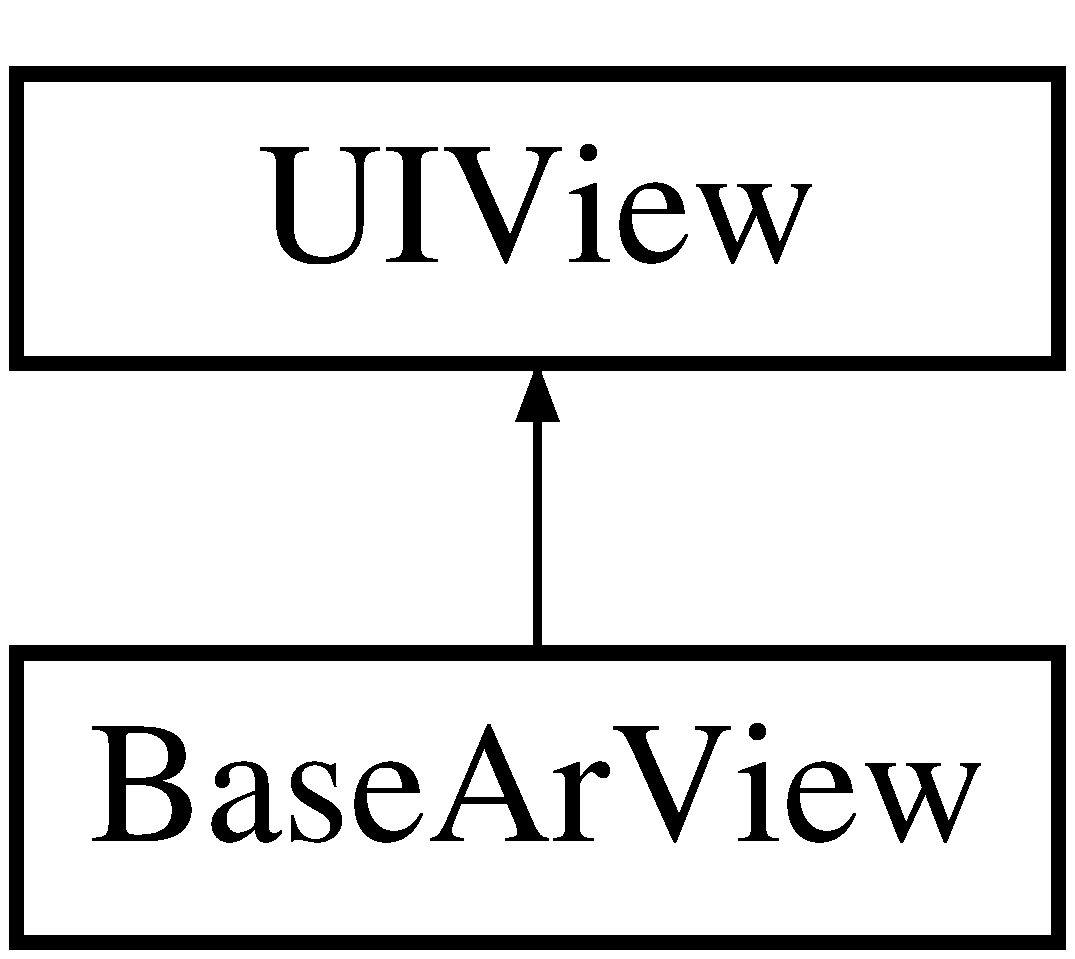
\includegraphics[height=2.000000cm]{d5/d64/interface_base_ar_view}
\end{center}
\end{figure}
\subsection*{Metody instance}
\begin{DoxyCompactItemize}
\item 
\hypertarget{interface_base_ar_view_aace15b18427bf737fd3c4273ae9e8c58}{(id) -\/ {\bfseries init\-With\-Frame\-And\-Capture\-Session\-:capture\-Session\-:}}\label{d5/d64/interface_base_ar_view_aace15b18427bf737fd3c4273ae9e8c58}

\item 
\hypertarget{interface_base_ar_view_a0e60ce8ce8fb1adc65ead18a2812a27a}{(void) -\/ {\bfseries append\-As\-Next\-Pipe\-:}}\label{d5/d64/interface_base_ar_view_a0e60ce8ce8fb1adc65ead18a2812a27a}

\item 
\hypertarget{interface_base_ar_view_ac69ba9a0fa58d9621f7e558c41f88471}{(void) -\/ {\bfseries show\-Preview\-Layer}}\label{d5/d64/interface_base_ar_view_ac69ba9a0fa58d9621f7e558c41f88471}

\item 
\hypertarget{interface_base_ar_view_ad94f53f246123743f7c754973e4a4be7}{(void) -\/ {\bfseries hide\-Preview\-Layer}}\label{d5/d64/interface_base_ar_view_ad94f53f246123743f7c754973e4a4be7}

\item 
\hypertarget{interface_base_ar_view_a89c6931f254b4d9a3e79f559bbc2ce35}{(void) -\/ {\bfseries show\-Frame\-Output}}\label{d5/d64/interface_base_ar_view_a89c6931f254b4d9a3e79f559bbc2ce35}

\item 
\hypertarget{interface_base_ar_view_a537347a63628e5c399ed2a610d005870}{(void) -\/ {\bfseries hide\-Frame\-Output}}\label{d5/d64/interface_base_ar_view_a537347a63628e5c399ed2a610d005870}

\item 
\hypertarget{interface_base_ar_view_aeddb63caed1e9a01863351898560af88}{(void) -\/ {\bfseries draw\-View\-:}}\label{d5/d64/interface_base_ar_view_aeddb63caed1e9a01863351898560af88}

\item 
\hypertarget{interface_base_ar_view_af54ad10be4020851537a750a5efefef0}{(\hyperlink{class_ar_pipe_1_1_pipe_output_connector}{Ar\-Pipe\-::\-Pipe\-Output\-Connector} $\ast$) -\/ {\bfseries pipe\-Connector}}\label{d5/d64/interface_base_ar_view_af54ad10be4020851537a750a5efefef0}

\end{DoxyCompactItemize}
\subsection*{Chráněné atributy}
\begin{DoxyCompactItemize}
\item 
\hypertarget{interface_base_ar_view_aee083bf02dd87f4479f1ca82de374aa8}{A\-V\-Capture\-Video\-Preview\-Layer $\ast$ {\bfseries preview\-Layer}}\label{d5/d64/interface_base_ar_view_aee083bf02dd87f4479f1ca82de374aa8}

\item 
\hypertarget{interface_base_ar_view_af6d719fef8d99c5fe86e64e236a8e20b}{\hyperlink{interface_g_l_view}{G\-L\-View} $\ast$ {\bfseries gl\-View}}\label{d5/d64/interface_base_ar_view_af6d719fef8d99c5fe86e64e236a8e20b}

\item 
\hypertarget{interface_base_ar_view_a5e822ab26b3730db244daab10e63244d}{U\-I\-View $\ast$ {\bfseries preview\-View}}\label{d5/d64/interface_base_ar_view_a5e822ab26b3730db244daab10e63244d}

\item 
\hypertarget{interface_base_ar_view_a365837b2f7c9e1a1428e7b2d6179e844}{\hyperlink{class_ar_pipe_1_1_pipe_output_connector}{Ar\-Pipe\-::\-Pipe\-Output\-Connector} $\ast$ {\bfseries connector}}\label{d5/d64/interface_base_ar_view_a365837b2f7c9e1a1428e7b2d6179e844}

\item 
\hypertarget{interface_base_ar_view_a1c6bcb43c046e236ff516e2e1fab41d0}{Boolean {\bfseries show\-Preview}}\label{d5/d64/interface_base_ar_view_a1c6bcb43c046e236ff516e2e1fab41d0}

\item 
\hypertarget{interface_base_ar_view_a82f0c58d3b54311a4f5e6800fb237f64}{Boolean {\bfseries display\-Link\-Supported}}\label{d5/d64/interface_base_ar_view_a82f0c58d3b54311a4f5e6800fb237f64}

\item 
\hypertarget{interface_base_ar_view_adf731ae38bf4ec76aff9d982cbf5e668}{N\-S\-Timer $\ast$ {\bfseries animation\-Timer}}\label{d5/d64/interface_base_ar_view_adf731ae38bf4ec76aff9d982cbf5e668}

\item 
\hypertarget{interface_base_ar_view_af3eec68bfde68e2541b7ee6ed4862241}{N\-S\-Integer {\bfseries frame\-Rate}}\label{d5/d64/interface_base_ar_view_af3eec68bfde68e2541b7ee6ed4862241}

\item 
\hypertarget{interface_base_ar_view_a3c1bb73d439b7597066db4ad9af46e47}{id {\bfseries display\-Link}}\label{d5/d64/interface_base_ar_view_a3c1bb73d439b7597066db4ad9af46e47}

\end{DoxyCompactItemize}
\subsection*{Vlastnosti}
\begin{DoxyCompactItemize}
\item 
\hypertarget{interface_base_ar_view_a8c28981c0e1982d5de9ff06241c01ead}{A\-V\-Capture\-Session $\ast$ {\bfseries session}}\label{d5/d64/interface_base_ar_view_a8c28981c0e1982d5de9ff06241c01ead}

\end{DoxyCompactItemize}


Dokumentace pro tuto třídu byla generována z následujících souborů\-:\begin{DoxyCompactItemize}
\item 
U\-I/Base\-Ar\-View.\-h\item 
U\-I/Base\-Ar\-View.\-mm\end{DoxyCompactItemize}

\hypertarget{class_ar_pipe_1_1_base_frame_container}{\section{Dokumentace třídy Ar\-Pipe\-:\-:Base\-Frame\-Container}
\label{da/d35/class_ar_pipe_1_1_base_frame_container}\index{Ar\-Pipe\-::\-Base\-Frame\-Container@{Ar\-Pipe\-::\-Base\-Frame\-Container}}
}
\subsection*{Veřejné metody}
\begin{DoxyCompactItemize}
\item 
\hypertarget{class_ar_pipe_1_1_base_frame_container_a473f29983266b94c82017782df89ce49}{{\bfseries Base\-Frame\-Container} (cv\-::\-Mat frame\-Mat)}\label{da/d35/class_ar_pipe_1_1_base_frame_container_a473f29983266b94c82017782df89ce49}

\item 
\hypertarget{class_ar_pipe_1_1_base_frame_container_ac7699fdd241a920e0e88a5f6f6ff5edc}{{\bfseries Base\-Frame\-Container} (\hyperlink{class_ar_pipe_1_1_frame}{Frame} $\ast$frm)}\label{da/d35/class_ar_pipe_1_1_base_frame_container_ac7699fdd241a920e0e88a5f6f6ff5edc}

\item 
\hypertarget{class_ar_pipe_1_1_base_frame_container_a789cc2cf1545414b1ef169f66cd908b7}{\hyperlink{class_ar_pipe_1_1_frame}{Frame} $\ast$ {\bfseries get\-Frame} ()}\label{da/d35/class_ar_pipe_1_1_base_frame_container_a789cc2cf1545414b1ef169f66cd908b7}

\item 
\hypertarget{class_ar_pipe_1_1_base_frame_container_af9a7c9b39dfd1d54a69b32e5bffbc1f6}{\hyperlink{class_ar_pipe_1_1_shapes}{Shapes} $\ast$ {\bfseries get\-Shapes} ()}\label{da/d35/class_ar_pipe_1_1_base_frame_container_af9a7c9b39dfd1d54a69b32e5bffbc1f6}

\item 
\hypertarget{class_ar_pipe_1_1_base_frame_container_acedbe9f0b649343f08753a77dcb80506}{\hyperlink{class_ar_pipe_1_1_base_frame_container}{Base\-Frame\-Container} $\ast$ {\bfseries clone} ()}\label{da/d35/class_ar_pipe_1_1_base_frame_container_acedbe9f0b649343f08753a77dcb80506}

\end{DoxyCompactItemize}
\subsection*{Chráněné atributy}
\begin{DoxyCompactItemize}
\item 
\hypertarget{class_ar_pipe_1_1_base_frame_container_adae12dc85967c31c9cf79bde5c6c48b7}{\hyperlink{class_ar_pipe_1_1_frame}{Frame} $\ast$ {\bfseries frame}}\label{da/d35/class_ar_pipe_1_1_base_frame_container_adae12dc85967c31c9cf79bde5c6c48b7}

\item 
\hypertarget{class_ar_pipe_1_1_base_frame_container_a02f4d9c206cc7231c403e72d68f91396}{\hyperlink{class_ar_pipe_1_1_shapes}{Shapes} $\ast$ {\bfseries shapes}}\label{da/d35/class_ar_pipe_1_1_base_frame_container_a02f4d9c206cc7231c403e72d68f91396}

\end{DoxyCompactItemize}


Dokumentace pro tuto třídu byla generována z následujících souborů\-:\begin{DoxyCompactItemize}
\item 
Model/Base\-Frame\-Container.\-h\item 
Model/Base\-Frame\-Container.\-cpp\end{DoxyCompactItemize}

\hypertarget{class_ar_pipe_1_1_base_frame_source}{\section{Dokumentace třídy Ar\-Pipe\-:\-:Base\-Frame\-Source}
\label{d6/d97/class_ar_pipe_1_1_base_frame_source}\index{Ar\-Pipe\-::\-Base\-Frame\-Source@{Ar\-Pipe\-::\-Base\-Frame\-Source}}
}
Diagram dědičnosti pro třídu Ar\-Pipe\-:\-:Base\-Frame\-Source\begin{figure}[H]
\begin{center}
\leavevmode
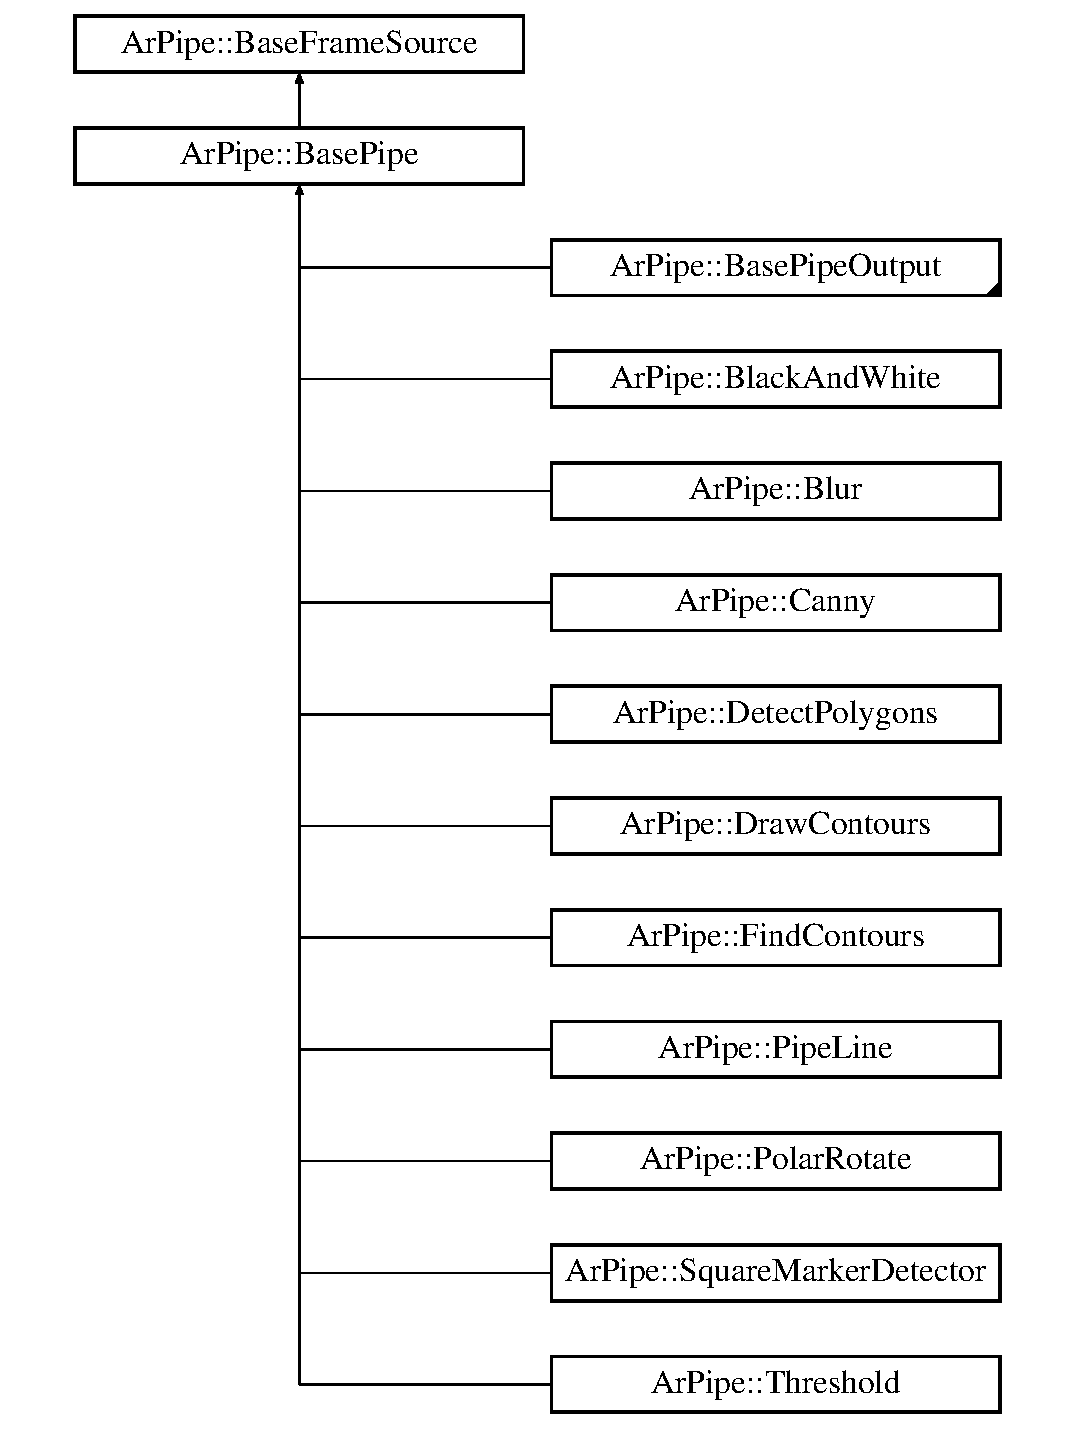
\includegraphics[height=12.000000cm]{d6/d97/class_ar_pipe_1_1_base_frame_source}
\end{center}
\end{figure}
\subsection*{Veřejné metody}
\begin{DoxyCompactItemize}
\item 
\hypertarget{class_ar_pipe_1_1_base_frame_source_a7930cb5e6a1a2bffd9217394e7f4faf4}{void {\bfseries add\-Next\-Pipe} (\hyperlink{class_ar_pipe_1_1_base_pipe}{Base\-Pipe} $\ast$pipe)}\label{d6/d97/class_ar_pipe_1_1_base_frame_source_a7930cb5e6a1a2bffd9217394e7f4faf4}

\item 
\hypertarget{class_ar_pipe_1_1_base_frame_source_a061c93c08b081c41f6a4845f20149e1a}{void {\bfseries push\-Frame\-Conainer\-To\-Next\-Pipes} (\hyperlink{class_ar_pipe_1_1_base_frame_container}{Base\-Frame\-Container} $\ast$container)}\label{d6/d97/class_ar_pipe_1_1_base_frame_source_a061c93c08b081c41f6a4845f20149e1a}

\end{DoxyCompactItemize}
\subsection*{Chráněné atributy}
\begin{DoxyCompactItemize}
\item 
\hypertarget{class_ar_pipe_1_1_base_frame_source_a095bf6e429526c21b16c111adec1a6ec}{std\-::vector$<$ \hyperlink{class_ar_pipe_1_1_base_pipe}{Base\-Pipe} $\ast$ $>$ {\bfseries next\-Pipes}}\label{d6/d97/class_ar_pipe_1_1_base_frame_source_a095bf6e429526c21b16c111adec1a6ec}

\end{DoxyCompactItemize}


Dokumentace pro tuto třídu byla generována z následujících souborů\-:\begin{DoxyCompactItemize}
\item 
Model/Base\-Frame\-Source.\-h\item 
Model/Base\-Frame\-Source.\-cpp\end{DoxyCompactItemize}

\hypertarget{class_ar_pipe_1_1_base_pipe}{\section{Dokumentace třídy Ar\-Pipe\-:\-:Base\-Pipe}
\label{dd/d99/class_ar_pipe_1_1_base_pipe}\index{Ar\-Pipe\-::\-Base\-Pipe@{Ar\-Pipe\-::\-Base\-Pipe}}
}
Diagram dědičnosti pro třídu Ar\-Pipe\-:\-:Base\-Pipe\begin{figure}[H]
\begin{center}
\leavevmode
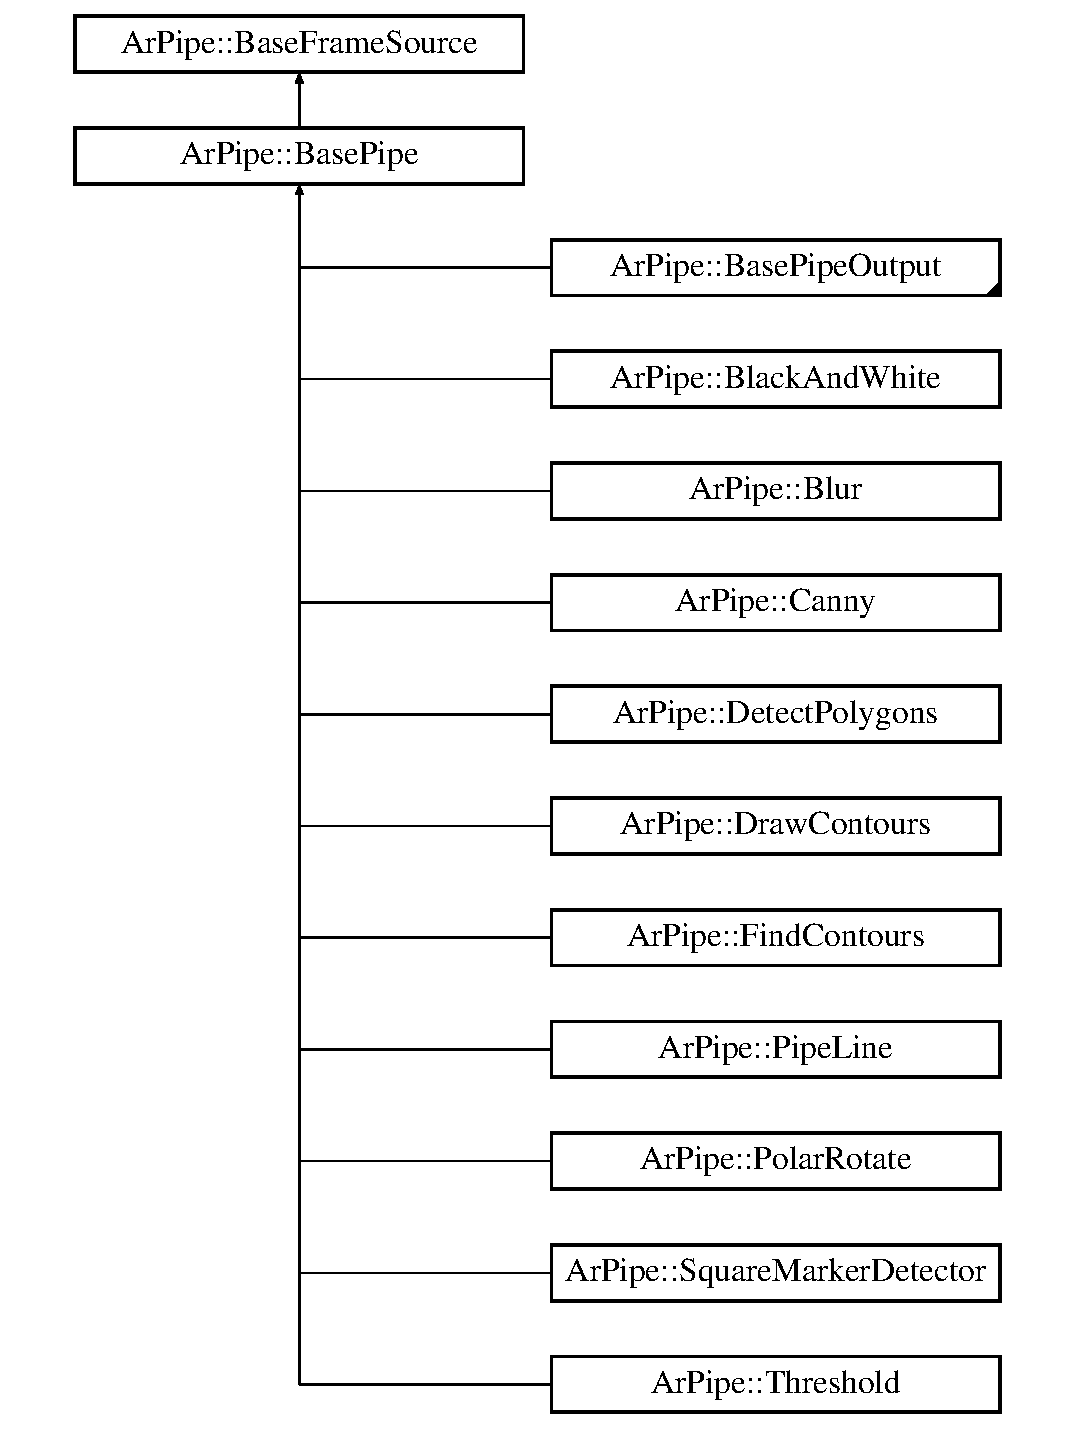
\includegraphics[height=12.000000cm]{dd/d99/class_ar_pipe_1_1_base_pipe}
\end{center}
\end{figure}
\subsection*{Veřejné metody}
\begin{DoxyCompactItemize}
\item 
\hypertarget{class_ar_pipe_1_1_base_pipe_af407d5fe6eae18597926f8fcb95f91e5}{{\bfseries Base\-Pipe} (\hyperlink{class_ar_pipe_1_1_base_frame_source}{Base\-Frame\-Source} $\ast$previous\-Pipe)}\label{dd/d99/class_ar_pipe_1_1_base_pipe_af407d5fe6eae18597926f8fcb95f91e5}

\item 
\hypertarget{class_ar_pipe_1_1_base_pipe_aeca79efb909fc6d29e26eecfa480c22f}{void {\bfseries push\-New\-Frame\-Container} (\hyperlink{class_ar_pipe_1_1_base_frame_container}{Base\-Frame\-Container} $\ast$frm, \hyperlink{class_ar_pipe_1_1_base_frame_source}{Base\-Frame\-Source} $\ast$frame\-Source)}\label{dd/d99/class_ar_pipe_1_1_base_pipe_aeca79efb909fc6d29e26eecfa480c22f}

\item 
\hypertarget{class_ar_pipe_1_1_base_pipe_ae7b3a04a3110e7ff5a9cac8da0ed7bc4}{virtual void {\bfseries process\-Frame\-Container} (\hyperlink{class_ar_pipe_1_1_base_frame_container}{Base\-Frame\-Container} $\ast$frm, \hyperlink{class_ar_pipe_1_1_base_frame_source}{Base\-Frame\-Source} $\ast$frame\-Source)}\label{dd/d99/class_ar_pipe_1_1_base_pipe_ae7b3a04a3110e7ff5a9cac8da0ed7bc4}

\item 
\hypertarget{class_ar_pipe_1_1_base_pipe_ace97703be27ecda02138dc4f1fe71abd}{{\footnotesize template$<$class T $>$ }\\T {\bfseries init} ()}\label{dd/d99/class_ar_pipe_1_1_base_pipe_ace97703be27ecda02138dc4f1fe71abd}

\end{DoxyCompactItemize}
\subsection*{Statické veřejné metody}
\begin{DoxyCompactItemize}
\item 
\hypertarget{class_ar_pipe_1_1_base_pipe_aaf3ffa50c0d4999062b925a5e7306844}{{\footnotesize template$<$class T $>$ }\\static T {\bfseries init} ()}\label{dd/d99/class_ar_pipe_1_1_base_pipe_aaf3ffa50c0d4999062b925a5e7306844}

\end{DoxyCompactItemize}
\subsection*{Další zděděné členy}


Dokumentace pro tuto třídu byla generována z následujících souborů\-:\begin{DoxyCompactItemize}
\item 
Model/Base\-Pipe.\-h\item 
Model/Base\-Pipe.\-cpp\end{DoxyCompactItemize}

\hypertarget{class_ar_pipe_1_1_base_pipe_output}{\section{Dokumentace třídy Ar\-Pipe\-:\-:Base\-Pipe\-Output}
\label{dd/dad/class_ar_pipe_1_1_base_pipe_output}\index{Ar\-Pipe\-::\-Base\-Pipe\-Output@{Ar\-Pipe\-::\-Base\-Pipe\-Output}}
}
Diagram dědičnosti pro třídu Ar\-Pipe\-:\-:Base\-Pipe\-Output\begin{figure}[H]
\begin{center}
\leavevmode
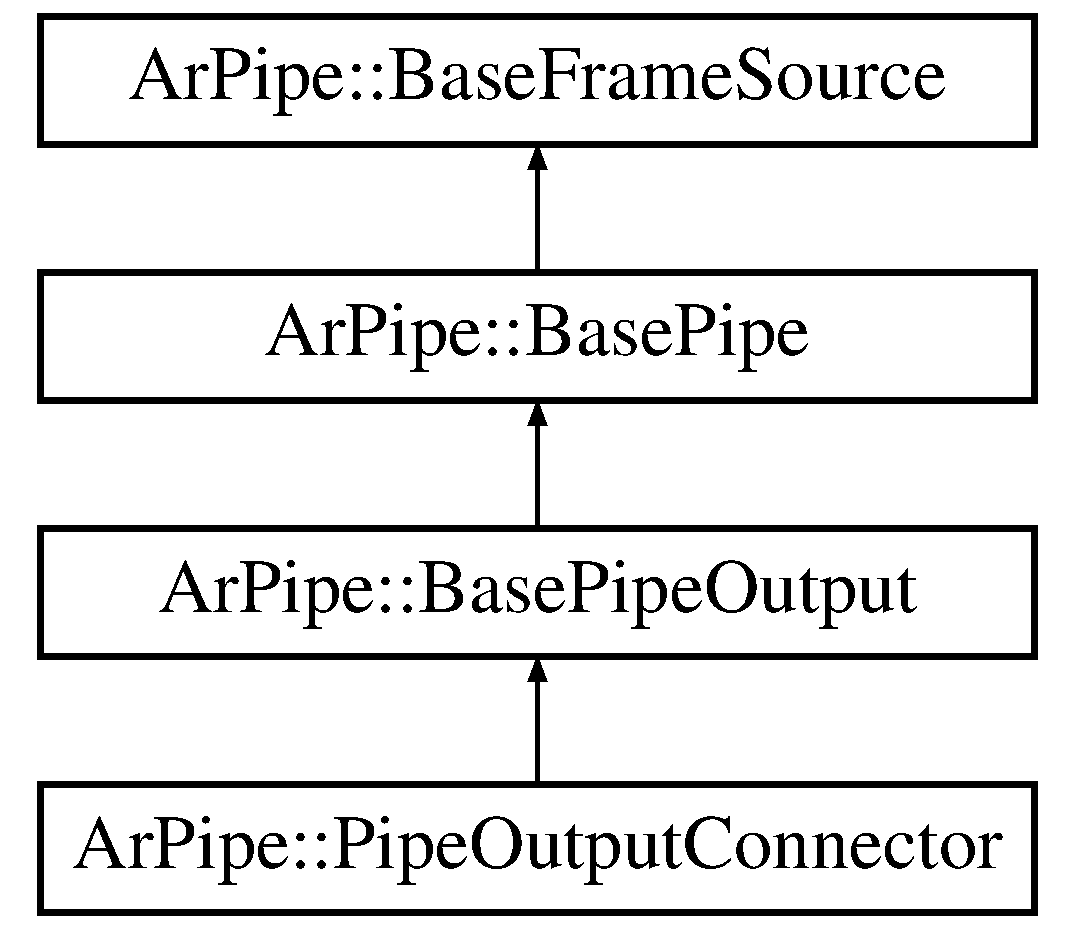
\includegraphics[height=4.000000cm]{dd/dad/class_ar_pipe_1_1_base_pipe_output}
\end{center}
\end{figure}
\subsection*{Další zděděné členy}


Dokumentace pro tuto třídu byla generována z následujícího souboru\-:\begin{DoxyCompactItemize}
\item 
Model/Base\-Pipe\-Output.\-h\end{DoxyCompactItemize}

\hypertarget{class_ar_pipe_1_1_black_and_white}{\section{Dokumentace třídy Ar\-Pipe\-:\-:Black\-And\-White}
\label{df/d31/class_ar_pipe_1_1_black_and_white}\index{Ar\-Pipe\-::\-Black\-And\-White@{Ar\-Pipe\-::\-Black\-And\-White}}
}
Diagram dědičnosti pro třídu Ar\-Pipe\-:\-:Black\-And\-White\begin{figure}[H]
\begin{center}
\leavevmode
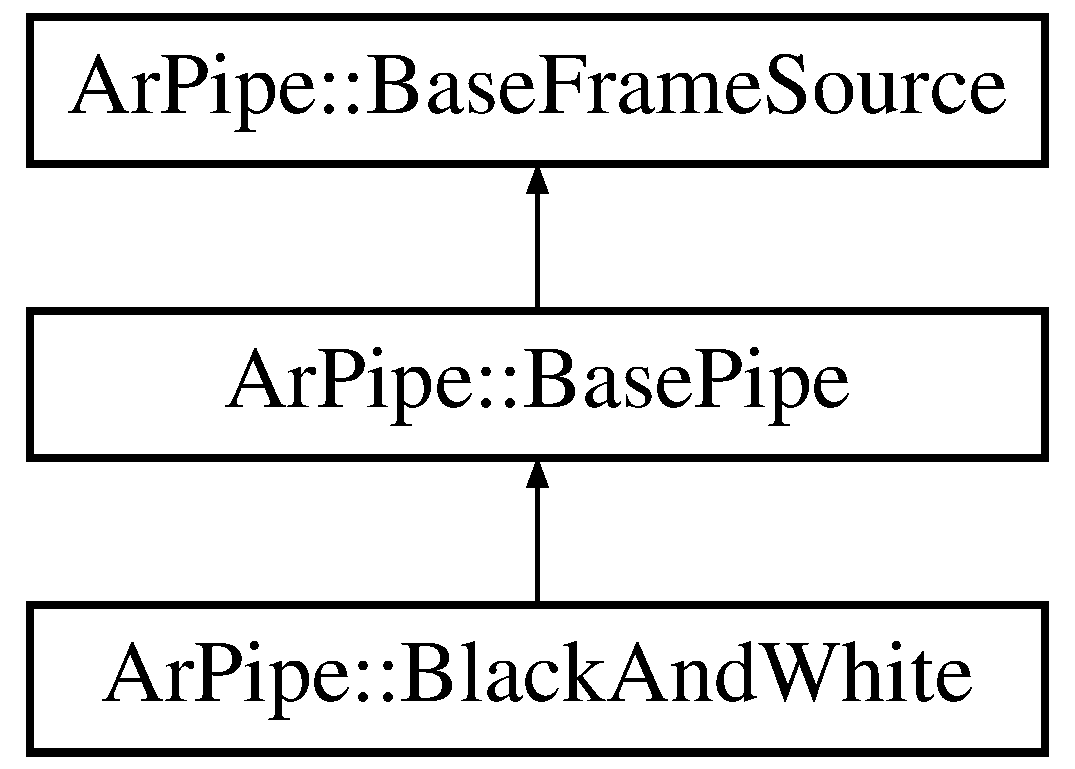
\includegraphics[height=3.000000cm]{df/d31/class_ar_pipe_1_1_black_and_white}
\end{center}
\end{figure}
\subsection*{Veřejné metody}
\begin{DoxyCompactItemize}
\item 
\hypertarget{class_ar_pipe_1_1_black_and_white_a7750c0842578069a60a29dfbf5c63356}{{\bfseries Black\-And\-White} (\hyperlink{class_ar_pipe_1_1_base_frame_source}{Base\-Frame\-Source} $\ast$previous\-Pipe)}\label{df/d31/class_ar_pipe_1_1_black_and_white_a7750c0842578069a60a29dfbf5c63356}

\item 
\hypertarget{class_ar_pipe_1_1_black_and_white_addb7f527851e0fa51c2bef8285591a62}{void {\bfseries process\-Frame\-Container} (\hyperlink{class_ar_pipe_1_1_base_frame_container}{Base\-Frame\-Container} $\ast$frm, \hyperlink{class_ar_pipe_1_1_base_frame_source}{Base\-Frame\-Source} $\ast$frame\-Source)}\label{df/d31/class_ar_pipe_1_1_black_and_white_addb7f527851e0fa51c2bef8285591a62}

\item 
\hypertarget{class_ar_pipe_1_1_black_and_white_a13a2d7b682bc12a94f12de7ce9b9f9f3}{\hyperlink{class_ar_pipe_1_1_black_and_white}{Black\-And\-White} $\ast$ {\bfseries to\-Color} ()}\label{df/d31/class_ar_pipe_1_1_black_and_white_a13a2d7b682bc12a94f12de7ce9b9f9f3}

\end{DoxyCompactItemize}
\subsection*{Statické veřejné metody}
\begin{DoxyCompactItemize}
\item 
\hypertarget{class_ar_pipe_1_1_black_and_white_a1acbe16ae97d80527a5dc4f286a172ee}{static \hyperlink{class_ar_pipe_1_1_black_and_white}{Black\-And\-White} $\ast$ {\bfseries init} ()}\label{df/d31/class_ar_pipe_1_1_black_and_white_a1acbe16ae97d80527a5dc4f286a172ee}

\end{DoxyCompactItemize}
\subsection*{Chráněné atributy}
\begin{DoxyCompactItemize}
\item 
\hypertarget{class_ar_pipe_1_1_black_and_white_a4814162cf5714b5bbebe3e4a69a19676}{bool {\bfseries color}}\label{df/d31/class_ar_pipe_1_1_black_and_white_a4814162cf5714b5bbebe3e4a69a19676}

\end{DoxyCompactItemize}


Dokumentace pro tuto třídu byla generována z následujících souborů\-:\begin{DoxyCompactItemize}
\item 
Pipes/\-Effects/Black\-And\-White.\-h\item 
Pipes/\-Effects/Black\-And\-White.\-cpp\end{DoxyCompactItemize}

\hypertarget{class_ar_pipe_1_1_blur}{\section{Dokumentace třídy Ar\-Pipe\-:\-:Blur}
\label{d1/df9/class_ar_pipe_1_1_blur}\index{Ar\-Pipe\-::\-Blur@{Ar\-Pipe\-::\-Blur}}
}
Diagram dědičnosti pro třídu Ar\-Pipe\-:\-:Blur\begin{figure}[H]
\begin{center}
\leavevmode
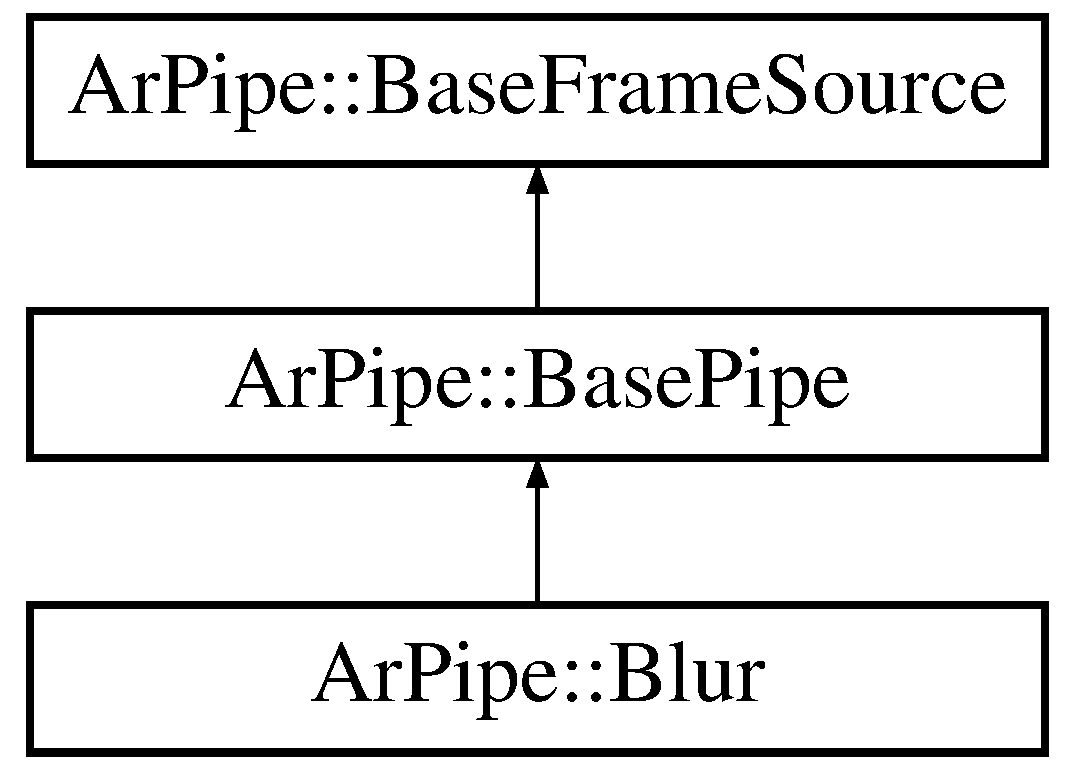
\includegraphics[height=3.000000cm]{d1/df9/class_ar_pipe_1_1_blur}
\end{center}
\end{figure}
\subsection*{Veřejné metody}
\begin{DoxyCompactItemize}
\item 
\hypertarget{class_ar_pipe_1_1_blur_a8f9e19aaa44b2333620ce10a70be6dc8}{{\bfseries Blur} (\hyperlink{class_ar_pipe_1_1_base_frame_source}{Base\-Frame\-Source} $\ast$previous\-Pipe)}\label{d1/df9/class_ar_pipe_1_1_blur_a8f9e19aaa44b2333620ce10a70be6dc8}

\item 
void \hyperlink{class_ar_pipe_1_1_blur_afd4bca524f1dff0d515308d7c22e93a9}{process\-Frame\-Container} (\hyperlink{class_ar_pipe_1_1_base_frame_container}{Base\-Frame\-Container} $\ast$frm, \hyperlink{class_ar_pipe_1_1_base_frame_source}{Base\-Frame\-Source} $\ast$frame\-Source)
\item 
\hypertarget{class_ar_pipe_1_1_blur_ac9a413eda8c4a52fa047c942788c3dd8}{\hyperlink{class_ar_pipe_1_1_blur}{Blur} $\ast$ {\bfseries set\-Type} (int type)}\label{d1/df9/class_ar_pipe_1_1_blur_ac9a413eda8c4a52fa047c942788c3dd8}

\item 
\hypertarget{class_ar_pipe_1_1_blur_a588e4beebabf621640f49528c3641435}{\hyperlink{class_ar_pipe_1_1_blur}{Blur} $\ast$ {\bfseries set\-Depth} (int depth)}\label{d1/df9/class_ar_pipe_1_1_blur_a588e4beebabf621640f49528c3641435}

\item 
\hypertarget{class_ar_pipe_1_1_blur_a9d2fc1475264e01315089bf84183509b}{\hyperlink{class_ar_pipe_1_1_blur}{Blur} $\ast$ {\bfseries set\-Type\-Gaussian} ()}\label{d1/df9/class_ar_pipe_1_1_blur_a9d2fc1475264e01315089bf84183509b}

\item 
\hypertarget{class_ar_pipe_1_1_blur_a9d0a0b03a56fb33e0200afb6d846c733}{\hyperlink{class_ar_pipe_1_1_blur}{Blur} $\ast$ {\bfseries set\-Type\-Median} ()}\label{d1/df9/class_ar_pipe_1_1_blur_a9d0a0b03a56fb33e0200afb6d846c733}

\item 
\hypertarget{class_ar_pipe_1_1_blur_a349fb13ca675d7d743d47722287ab33d}{\hyperlink{class_ar_pipe_1_1_blur}{Blur} $\ast$ {\bfseries set\-Type\-Bilateral} ()}\label{d1/df9/class_ar_pipe_1_1_blur_a349fb13ca675d7d743d47722287ab33d}

\end{DoxyCompactItemize}
\subsection*{Statické veřejné metody}
\begin{DoxyCompactItemize}
\item 
\hypertarget{class_ar_pipe_1_1_blur_ad4aa0c1151bd29d6e9cccfa82d8eb063}{static \hyperlink{class_ar_pipe_1_1_blur}{Blur} $\ast$ {\bfseries init} ()}\label{d1/df9/class_ar_pipe_1_1_blur_ad4aa0c1151bd29d6e9cccfa82d8eb063}

\item 
\hypertarget{class_ar_pipe_1_1_blur_a47e5a6d2c7d247538f069cfef75434f4}{static \hyperlink{class_ar_pipe_1_1_blur}{Blur} $\ast$ {\bfseries init} (int depth)}\label{d1/df9/class_ar_pipe_1_1_blur_a47e5a6d2c7d247538f069cfef75434f4}

\end{DoxyCompactItemize}
\subsection*{Chráněné typy}
\begin{DoxyCompactItemize}
\item 
enum \{ {\bfseries A\-R\-P\-\_\-\-B\-L\-U\-R\-\_\-\-S\-T\-A\-N\-D\-A\-R\-D}, 
{\bfseries A\-R\-P\-\_\-\-B\-L\-U\-R\-\_\-\-G\-A\-U\-S\-S\-I\-A\-N}, 
{\bfseries A\-R\-P\-\_\-\-B\-L\-U\-R\-\_\-\-M\-E\-D\-I\-A\-N}, 
{\bfseries A\-R\-P\-\_\-\-B\-L\-U\-R\-\_\-\-B\-I\-L\-A\-T\-E\-R\-A\-L}
 \}
\end{DoxyCompactItemize}
\subsection*{Chráněné atributy}
\begin{DoxyCompactItemize}
\item 
\hypertarget{class_ar_pipe_1_1_blur_a5dd8d1e00f61f3544a67a936361eb970}{int {\bfseries kernel\-Length}}\label{d1/df9/class_ar_pipe_1_1_blur_a5dd8d1e00f61f3544a67a936361eb970}

\item 
\hypertarget{class_ar_pipe_1_1_blur_a341dc684c8555c62e28a408c5920bb63}{enum Ar\-Pipe\-::\-Blur\-:: \{ ... \}  {\bfseries type}}\label{d1/df9/class_ar_pipe_1_1_blur_a341dc684c8555c62e28a408c5920bb63}

\end{DoxyCompactItemize}


\subsection{Dokumentace k metodám}
\hypertarget{class_ar_pipe_1_1_blur_afd4bca524f1dff0d515308d7c22e93a9}{\index{Ar\-Pipe\-::\-Blur@{Ar\-Pipe\-::\-Blur}!process\-Frame\-Container@{process\-Frame\-Container}}
\index{process\-Frame\-Container@{process\-Frame\-Container}!ArPipe::Blur@{Ar\-Pipe\-::\-Blur}}
\subsubsection[{process\-Frame\-Container}]{\setlength{\rightskip}{0pt plus 5cm}void Ar\-Pipe\-::\-Blur\-::process\-Frame\-Container (
\begin{DoxyParamCaption}
\item[{{\bf Base\-Frame\-Container} $\ast$}]{frm, }
\item[{{\bf Base\-Frame\-Source} $\ast$}]{frame\-Source}
\end{DoxyParamCaption}
)\hspace{0.3cm}{\ttfamily [virtual]}}}\label{d1/df9/class_ar_pipe_1_1_blur_afd4bca524f1dff0d515308d7c22e93a9}
Applying Homogeneous blur

Applying Gaussian blur

Applying Median blur

Applying Bilateral Filter 

Reimplementuje stejnojmenný prvek z \hyperlink{class_ar_pipe_1_1_base_pipe}{Ar\-Pipe\-::\-Base\-Pipe}.



Dokumentace pro tuto třídu byla generována z následujících souborů\-:\begin{DoxyCompactItemize}
\item 
Pipes/\-Effects/Blur.\-h\item 
Pipes/\-Effects/Blur.\-cpp\end{DoxyCompactItemize}

\hypertarget{interface_camera_frame_source}{\section{Dokumentace třídy Camera\-Frame\-Source}
\label{db/dad/interface_camera_frame_source}\index{Camera\-Frame\-Source@{Camera\-Frame\-Source}}
}
Diagram dědičnosti pro třídu Camera\-Frame\-Source\begin{figure}[H]
\begin{center}
\leavevmode
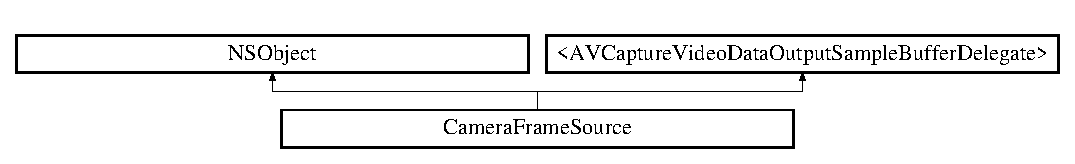
\includegraphics[height=1.755486cm]{db/dad/interface_camera_frame_source}
\end{center}
\end{figure}
\subsection*{Metody instance}
\begin{DoxyCompactItemize}
\item 
\hypertarget{interface_camera_frame_source_a05f4a47427d18144c0a2569db43ac337}{(\hyperlink{interface_camera_frame_source}{Camera\-Frame\-Source} $\ast$) -\/ {\bfseries init}}\label{db/dad/interface_camera_frame_source_a05f4a47427d18144c0a2569db43ac337}

\item 
\hypertarget{interface_camera_frame_source_a40ad8bd44e575a186f6ba5af67788312}{(void) -\/ {\bfseries start}}\label{db/dad/interface_camera_frame_source_a40ad8bd44e575a186f6ba5af67788312}

\item 
\hypertarget{interface_camera_frame_source_a68592d8757b77020ad1070631e3f30ee}{(void) -\/ {\bfseries stop}}\label{db/dad/interface_camera_frame_source_a68592d8757b77020ad1070631e3f30ee}

\item 
\hypertarget{interface_camera_frame_source_ac3d33c3ba7a81860c470ede51d46e2ba}{(void) -\/ {\bfseries set\-Next\-Pipe\-:}}\label{db/dad/interface_camera_frame_source_ac3d33c3ba7a81860c470ede51d46e2ba}

\item 
\hypertarget{interface_camera_frame_source_a67ad083cf405ccb4efc57232c2c8c298}{(A\-V\-Capture\-Session $\ast$) -\/ {\bfseries capture\-Session}}\label{db/dad/interface_camera_frame_source_a67ad083cf405ccb4efc57232c2c8c298}

\item 
\hypertarget{interface_camera_frame_source_a07057a809be7d76563d0e7dbb0d6fd1a}{(\hyperlink{class_ar_pipe_1_1_base_frame_source}{Ar\-Pipe\-::\-Base\-Frame\-Source} $\ast$) -\/ {\bfseries frame\-Source}}\label{db/dad/interface_camera_frame_source_a07057a809be7d76563d0e7dbb0d6fd1a}

\end{DoxyCompactItemize}
\subsection*{Chráněné atributy}
\begin{DoxyCompactItemize}
\item 
\hypertarget{interface_camera_frame_source_a8eea6afabc799bc7383407b367d03433}{A\-V\-Capture\-Session $\ast$ {\bfseries capture\-Session}}\label{db/dad/interface_camera_frame_source_a8eea6afabc799bc7383407b367d03433}

\item 
\hypertarget{interface_camera_frame_source_a7ee378581e57a4df8ca9d78264adfa06}{\hyperlink{class_ar_pipe_1_1_base_frame_source}{Ar\-Pipe\-::\-Base\-Frame\-Source} $\ast$ {\bfseries frame\-Source}}\label{db/dad/interface_camera_frame_source_a7ee378581e57a4df8ca9d78264adfa06}

\end{DoxyCompactItemize}


Dokumentace pro tuto třídu byla generována z následujících souborů\-:\begin{DoxyCompactItemize}
\item 
i\-O\-S\-Connectors/Camera\-Frame\-Source.\-h\item 
i\-O\-S\-Connectors/Camera\-Frame\-Source.\-mm\end{DoxyCompactItemize}

\hypertarget{classaruco_1_1_camera_parameters}{\section{Dokumentace třídy aruco\-:\-:Camera\-Parameters}
\label{d6/d88/classaruco_1_1_camera_parameters}\index{aruco\-::\-Camera\-Parameters@{aruco\-::\-Camera\-Parameters}}
}


Parameters of the camera.  




{\ttfamily \#include $<$cameraparameters.\-h$>$}

\subsection*{Veřejné metody}
\begin{DoxyCompactItemize}
\item 
\hyperlink{classaruco_1_1_camera_parameters_a23e30ef777f22f819a332592bf3db075}{Camera\-Parameters} ()
\item 
\hyperlink{classaruco_1_1_camera_parameters_a8abee4cd106b36900f0860b39ea7ef2a}{Camera\-Parameters} (cv\-::\-Mat camera\-Matrix, cv\-::\-Mat distorsion\-Coeff, cv\-::\-Size size)  throw (cv\-::\-Exception)
\item 
void \hyperlink{classaruco_1_1_camera_parameters_af51ad02ac8a968ed20161baa18ca6435}{set\-Params} (cv\-::\-Mat camera\-Matrix, cv\-::\-Mat distorsion\-Coeff, cv\-::\-Size size)  throw (cv\-::\-Exception)
\item 
\hyperlink{classaruco_1_1_camera_parameters_a9f9c0c3a68c29f3f5dd2b718de5217e1}{Camera\-Parameters} (const \hyperlink{classaruco_1_1_camera_parameters}{Camera\-Parameters} \&C\-I)
\item 
bool \hyperlink{classaruco_1_1_camera_parameters_ac3c1dde80f97886a1dc04c0439959596}{is\-Valid} () const 
\item 
\hyperlink{classaruco_1_1_camera_parameters}{Camera\-Parameters} \& \hyperlink{classaruco_1_1_camera_parameters_a4c13267368caccb7d05e79769460e1b3}{operator=} (const \hyperlink{classaruco_1_1_camera_parameters}{Camera\-Parameters} \&C\-I)
\item 
void \hyperlink{classaruco_1_1_camera_parameters_a65062b40124245d0386a365189ce86bc}{read\-From\-File} (string path)  throw (cv\-::\-Exception)
\item 
void \hyperlink{classaruco_1_1_camera_parameters_a0fb7e36dcc255b6d8f6cb191bf5bb635}{save\-To\-File} (string path, bool in\-X\-M\-L=true)  throw (cv\-::\-Exception)
\item 
void \hyperlink{classaruco_1_1_camera_parameters_a866dbc61304f56166da41220e94f4f0f}{read\-From\-X\-M\-L\-File} (string file\-Path)  throw (cv\-::\-Exception)
\item 
void \hyperlink{classaruco_1_1_camera_parameters_aabf139725fb75759b4172a53de63100f}{resize} (cv\-::\-Size size)  throw (cv\-::\-Exception)
\item 
void \hyperlink{classaruco_1_1_camera_parameters_adbfb82ecadfbe6c59c47798f558064ac}{gl\-Get\-Projection\-Matrix} (cv\-::\-Size org\-Img\-Size, cv\-::\-Size size, double proj\-\_\-matrix\mbox{[}16\mbox{]}, double gnear, double gfar, bool invert=false)  throw (cv\-::\-Exception)
\item 
void \hyperlink{classaruco_1_1_camera_parameters_adb5924aaec7e149ba5ea509158663540}{Ogre\-Get\-Projection\-Matrix} (cv\-::\-Size org\-Img\-Size, cv\-::\-Size size, double proj\-\_\-matrix\mbox{[}16\mbox{]}, double gnear, double gfar, bool invert=false)  throw (cv\-::\-Exception)
\end{DoxyCompactItemize}
\subsection*{Statické veřejné metody}
\begin{DoxyCompactItemize}
\item 
static cv\-::\-Point3f \hyperlink{classaruco_1_1_camera_parameters_ab3f102b448814ed007788d9d6020beb2}{get\-Camera\-Location} (cv\-::\-Mat Rvec, cv\-::\-Mat Tvec)
\end{DoxyCompactItemize}
\subsection*{Veřejné atributy}
\begin{DoxyCompactItemize}
\item 
\hypertarget{classaruco_1_1_camera_parameters_a5210f7dd5f0f4f0fea728357005d6bcd}{cv\-::\-Mat {\bfseries Camera\-Matrix}}\label{d6/d88/classaruco_1_1_camera_parameters_a5210f7dd5f0f4f0fea728357005d6bcd}

\item 
\hypertarget{classaruco_1_1_camera_parameters_a33a5ab0b2f00a4753a2fda307e24360a}{cv\-::\-Mat {\bfseries Distorsion}}\label{d6/d88/classaruco_1_1_camera_parameters_a33a5ab0b2f00a4753a2fda307e24360a}

\item 
\hypertarget{classaruco_1_1_camera_parameters_a08fdd4888daf7140cf31bdd341c3f303}{cv\-::\-Size {\bfseries Cam\-Size}}\label{d6/d88/classaruco_1_1_camera_parameters_a08fdd4888daf7140cf31bdd341c3f303}

\end{DoxyCompactItemize}


\subsection{Detailní popis}
Parameters of the camera. 

\subsection{Dokumentace konstruktoru a destruktoru}
\hypertarget{classaruco_1_1_camera_parameters_a23e30ef777f22f819a332592bf3db075}{\index{aruco\-::\-Camera\-Parameters@{aruco\-::\-Camera\-Parameters}!Camera\-Parameters@{Camera\-Parameters}}
\index{Camera\-Parameters@{Camera\-Parameters}!aruco::CameraParameters@{aruco\-::\-Camera\-Parameters}}
\subsubsection[{Camera\-Parameters}]{\setlength{\rightskip}{0pt plus 5cm}aruco\-::\-Camera\-Parameters\-::\-Camera\-Parameters (
\begin{DoxyParamCaption}
{}
\end{DoxyParamCaption}
)}}\label{d6/d88/classaruco_1_1_camera_parameters_a23e30ef777f22f819a332592bf3db075}
Empty constructor \hypertarget{classaruco_1_1_camera_parameters_a8abee4cd106b36900f0860b39ea7ef2a}{\index{aruco\-::\-Camera\-Parameters@{aruco\-::\-Camera\-Parameters}!Camera\-Parameters@{Camera\-Parameters}}
\index{Camera\-Parameters@{Camera\-Parameters}!aruco::CameraParameters@{aruco\-::\-Camera\-Parameters}}
\subsubsection[{Camera\-Parameters}]{\setlength{\rightskip}{0pt plus 5cm}aruco\-::\-Camera\-Parameters\-::\-Camera\-Parameters (
\begin{DoxyParamCaption}
\item[{cv\-::\-Mat}]{camera\-Matrix, }
\item[{cv\-::\-Mat}]{distorsion\-Coeff, }
\item[{cv\-::\-Size}]{size}
\end{DoxyParamCaption}
)  throw (cv\-::\-Exception)}}\label{d6/d88/classaruco_1_1_camera_parameters_a8abee4cd106b36900f0860b39ea7ef2a}
Creates the object from the info passed 
\begin{DoxyParams}{Parametry}
{\em camera\-Matrix} & 3x3 matrix (fx 0 cx, 0 fy cy, 0 0 1) \\
\hline
{\em distorsion\-Coeff} & 4x1 matrix (k1,k2,p1,p2) \\
\hline
{\em size} & image size \\
\hline
\end{DoxyParams}
\hypertarget{classaruco_1_1_camera_parameters_a9f9c0c3a68c29f3f5dd2b718de5217e1}{\index{aruco\-::\-Camera\-Parameters@{aruco\-::\-Camera\-Parameters}!Camera\-Parameters@{Camera\-Parameters}}
\index{Camera\-Parameters@{Camera\-Parameters}!aruco::CameraParameters@{aruco\-::\-Camera\-Parameters}}
\subsubsection[{Camera\-Parameters}]{\setlength{\rightskip}{0pt plus 5cm}aruco\-::\-Camera\-Parameters\-::\-Camera\-Parameters (
\begin{DoxyParamCaption}
\item[{const {\bf Camera\-Parameters} \&}]{C\-I}
\end{DoxyParamCaption}
)}}\label{d6/d88/classaruco_1_1_camera_parameters_a9f9c0c3a68c29f3f5dd2b718de5217e1}
Copy constructor 

\subsection{Dokumentace k metodám}
\hypertarget{classaruco_1_1_camera_parameters_ab3f102b448814ed007788d9d6020beb2}{\index{aruco\-::\-Camera\-Parameters@{aruco\-::\-Camera\-Parameters}!get\-Camera\-Location@{get\-Camera\-Location}}
\index{get\-Camera\-Location@{get\-Camera\-Location}!aruco::CameraParameters@{aruco\-::\-Camera\-Parameters}}
\subsubsection[{get\-Camera\-Location}]{\setlength{\rightskip}{0pt plus 5cm}cv\-::\-Point3f aruco\-::\-Camera\-Parameters\-::get\-Camera\-Location (
\begin{DoxyParamCaption}
\item[{cv\-::\-Mat}]{Rvec, }
\item[{cv\-::\-Mat}]{Tvec}
\end{DoxyParamCaption}
)\hspace{0.3cm}{\ttfamily [static]}}}\label{d6/d88/classaruco_1_1_camera_parameters_ab3f102b448814ed007788d9d6020beb2}
Returns the location of the camera in the reference system given by the rotation and translation vectors passed N\-O\-T T\-E\-S\-T\-E\-D \hypertarget{classaruco_1_1_camera_parameters_adbfb82ecadfbe6c59c47798f558064ac}{\index{aruco\-::\-Camera\-Parameters@{aruco\-::\-Camera\-Parameters}!gl\-Get\-Projection\-Matrix@{gl\-Get\-Projection\-Matrix}}
\index{gl\-Get\-Projection\-Matrix@{gl\-Get\-Projection\-Matrix}!aruco::CameraParameters@{aruco\-::\-Camera\-Parameters}}
\subsubsection[{gl\-Get\-Projection\-Matrix}]{\setlength{\rightskip}{0pt plus 5cm}void aruco\-::\-Camera\-Parameters\-::gl\-Get\-Projection\-Matrix (
\begin{DoxyParamCaption}
\item[{cv\-::\-Size}]{org\-Img\-Size, }
\item[{cv\-::\-Size}]{size, }
\item[{double}]{proj\-\_\-matrix\mbox{[}16\mbox{]}, }
\item[{double}]{gnear, }
\item[{double}]{gfar, }
\item[{bool}]{invert = {\ttfamily false}}
\end{DoxyParamCaption}
)  throw (cv\-::\-Exception)}}\label{d6/d88/classaruco_1_1_camera_parameters_adbfb82ecadfbe6c59c47798f558064ac}
Given the intrinsic camera parameters returns the G\-L\-\_\-\-P\-R\-O\-J\-E\-C\-T\-I\-O\-N matrix for opengl. P\-Lease N\-O\-T\-E that when using Open\-G\-L, it is assumed no camera distorsion! So, if it is not true, you should have undistor image


\begin{DoxyParams}{Parametry}
{\em org\-Img\-Size} & size of the original image \\
\hline
{\em size} & of the image/window where to render (can be different from the real camera image). Please not that it must be related to Cam\-Matrix \\
\hline
{\em proj\-\_\-matrix} & output projection matrix to give to opengl \\
\hline
{\em gnear,gfar,\-:} & visible rendering range \\
\hline
{\em invert,\-:} & indicates if the output projection matrix has to yield a horizontally inverted image because image data has not been stored in the order of gl\-Draw\-Pixels\-: bottom-\/to-\/top. \\
\hline
\end{DoxyParams}
\hypertarget{classaruco_1_1_camera_parameters_ac3c1dde80f97886a1dc04c0439959596}{\index{aruco\-::\-Camera\-Parameters@{aruco\-::\-Camera\-Parameters}!is\-Valid@{is\-Valid}}
\index{is\-Valid@{is\-Valid}!aruco::CameraParameters@{aruco\-::\-Camera\-Parameters}}
\subsubsection[{is\-Valid}]{\setlength{\rightskip}{0pt plus 5cm}bool aruco\-::\-Camera\-Parameters\-::is\-Valid (
\begin{DoxyParamCaption}
{}
\end{DoxyParamCaption}
) const\hspace{0.3cm}{\ttfamily [inline]}}}\label{d6/d88/classaruco_1_1_camera_parameters_ac3c1dde80f97886a1dc04c0439959596}
Indicates whether this object is valid \hypertarget{classaruco_1_1_camera_parameters_adb5924aaec7e149ba5ea509158663540}{\index{aruco\-::\-Camera\-Parameters@{aruco\-::\-Camera\-Parameters}!Ogre\-Get\-Projection\-Matrix@{Ogre\-Get\-Projection\-Matrix}}
\index{Ogre\-Get\-Projection\-Matrix@{Ogre\-Get\-Projection\-Matrix}!aruco::CameraParameters@{aruco\-::\-Camera\-Parameters}}
\subsubsection[{Ogre\-Get\-Projection\-Matrix}]{\setlength{\rightskip}{0pt plus 5cm}void aruco\-::\-Camera\-Parameters\-::\-Ogre\-Get\-Projection\-Matrix (
\begin{DoxyParamCaption}
\item[{cv\-::\-Size}]{org\-Img\-Size, }
\item[{cv\-::\-Size}]{size, }
\item[{double}]{proj\-\_\-matrix\mbox{[}16\mbox{]}, }
\item[{double}]{gnear, }
\item[{double}]{gfar, }
\item[{bool}]{invert = {\ttfamily false}}
\end{DoxyParamCaption}
)  throw (cv\-::\-Exception)}}\label{d6/d88/classaruco_1_1_camera_parameters_adb5924aaec7e149ba5ea509158663540}
setup camera for an Ogre project. Use\-: ... Ogre\-::\-Matrix4 P\-M(proj\-\_\-matrix\mbox{[}0\mbox{]}, proj\-\_\-matrix\mbox{[}1\mbox{]}, ... , proj\-\_\-matrix\mbox{[}15\mbox{]}); your\-Camera-\/$>$set\-Custom\-Projection\-Matrix(true, P\-M); your\-Camera-\/$>$set\-Custom\-View\-Matrix(true, Ogre\-::\-Matrix4\-::\-I\-D\-E\-N\-T\-I\-T\-Y); ... As in Open\-G\-L, it assumes no camera distorsion \hypertarget{classaruco_1_1_camera_parameters_a4c13267368caccb7d05e79769460e1b3}{\index{aruco\-::\-Camera\-Parameters@{aruco\-::\-Camera\-Parameters}!operator=@{operator=}}
\index{operator=@{operator=}!aruco::CameraParameters@{aruco\-::\-Camera\-Parameters}}
\subsubsection[{operator=}]{\setlength{\rightskip}{0pt plus 5cm}{\bf Camera\-Parameters} \& aruco\-::\-Camera\-Parameters\-::operator= (
\begin{DoxyParamCaption}
\item[{const {\bf Camera\-Parameters} \&}]{C\-I}
\end{DoxyParamCaption}
)}}\label{d6/d88/classaruco_1_1_camera_parameters_a4c13267368caccb7d05e79769460e1b3}
Assign operator \hypertarget{classaruco_1_1_camera_parameters_a65062b40124245d0386a365189ce86bc}{\index{aruco\-::\-Camera\-Parameters@{aruco\-::\-Camera\-Parameters}!read\-From\-File@{read\-From\-File}}
\index{read\-From\-File@{read\-From\-File}!aruco::CameraParameters@{aruco\-::\-Camera\-Parameters}}
\subsubsection[{read\-From\-File}]{\setlength{\rightskip}{0pt plus 5cm}void aruco\-::\-Camera\-Parameters\-::read\-From\-File (
\begin{DoxyParamCaption}
\item[{string}]{path}
\end{DoxyParamCaption}
)  throw (cv\-::\-Exception)}}\label{d6/d88/classaruco_1_1_camera_parameters_a65062b40124245d0386a365189ce86bc}
Reads the camera parameters from a file generated using save\-To\-File.

Reads the camera parameters from file \hypertarget{classaruco_1_1_camera_parameters_a866dbc61304f56166da41220e94f4f0f}{\index{aruco\-::\-Camera\-Parameters@{aruco\-::\-Camera\-Parameters}!read\-From\-X\-M\-L\-File@{read\-From\-X\-M\-L\-File}}
\index{read\-From\-X\-M\-L\-File@{read\-From\-X\-M\-L\-File}!aruco::CameraParameters@{aruco\-::\-Camera\-Parameters}}
\subsubsection[{read\-From\-X\-M\-L\-File}]{\setlength{\rightskip}{0pt plus 5cm}void aruco\-::\-Camera\-Parameters\-::read\-From\-X\-M\-L\-File (
\begin{DoxyParamCaption}
\item[{string}]{file\-Path}
\end{DoxyParamCaption}
)  throw (cv\-::\-Exception)}}\label{d6/d88/classaruco_1_1_camera_parameters_a866dbc61304f56166da41220e94f4f0f}
Reads from a Y\-A\-M\-L file generated with the opencv2.\-2 calibration utility \hypertarget{classaruco_1_1_camera_parameters_aabf139725fb75759b4172a53de63100f}{\index{aruco\-::\-Camera\-Parameters@{aruco\-::\-Camera\-Parameters}!resize@{resize}}
\index{resize@{resize}!aruco::CameraParameters@{aruco\-::\-Camera\-Parameters}}
\subsubsection[{resize}]{\setlength{\rightskip}{0pt plus 5cm}void aruco\-::\-Camera\-Parameters\-::resize (
\begin{DoxyParamCaption}
\item[{cv\-::\-Size}]{size}
\end{DoxyParamCaption}
)  throw (cv\-::\-Exception)}}\label{d6/d88/classaruco_1_1_camera_parameters_aabf139725fb75759b4172a53de63100f}
Adjust the parameters to the size of the image indicated \hypertarget{classaruco_1_1_camera_parameters_a0fb7e36dcc255b6d8f6cb191bf5bb635}{\index{aruco\-::\-Camera\-Parameters@{aruco\-::\-Camera\-Parameters}!save\-To\-File@{save\-To\-File}}
\index{save\-To\-File@{save\-To\-File}!aruco::CameraParameters@{aruco\-::\-Camera\-Parameters}}
\subsubsection[{save\-To\-File}]{\setlength{\rightskip}{0pt plus 5cm}void aruco\-::\-Camera\-Parameters\-::save\-To\-File (
\begin{DoxyParamCaption}
\item[{string}]{path, }
\item[{bool}]{in\-X\-M\-L = {\ttfamily true}}
\end{DoxyParamCaption}
)  throw (cv\-::\-Exception)}}\label{d6/d88/classaruco_1_1_camera_parameters_a0fb7e36dcc255b6d8f6cb191bf5bb635}
Saves this to a file \hypertarget{classaruco_1_1_camera_parameters_af51ad02ac8a968ed20161baa18ca6435}{\index{aruco\-::\-Camera\-Parameters@{aruco\-::\-Camera\-Parameters}!set\-Params@{set\-Params}}
\index{set\-Params@{set\-Params}!aruco::CameraParameters@{aruco\-::\-Camera\-Parameters}}
\subsubsection[{set\-Params}]{\setlength{\rightskip}{0pt plus 5cm}void aruco\-::\-Camera\-Parameters\-::set\-Params (
\begin{DoxyParamCaption}
\item[{cv\-::\-Mat}]{camera\-Matrix, }
\item[{cv\-::\-Mat}]{distorsion\-Coeff, }
\item[{cv\-::\-Size}]{size}
\end{DoxyParamCaption}
)  throw (cv\-::\-Exception)}}\label{d6/d88/classaruco_1_1_camera_parameters_af51ad02ac8a968ed20161baa18ca6435}
Sets the parameters 
\begin{DoxyParams}{Parametry}
{\em camera\-Matrix} & 3x3 matrix (fx 0 cx, 0 fy cy, 0 0 1) \\
\hline
{\em distorsion\-Coeff} & 4x1 matrix (k1,k2,p1,p2) \\
\hline
{\em size} & image size \\
\hline
\end{DoxyParams}


Dokumentace pro tuto třídu byla generována z následujících souborů\-:\begin{DoxyCompactItemize}
\item 
Aruco\-Utils/cameraparameters.\-h\item 
Aruco\-Utils/cameraparameters.\-cpp\end{DoxyCompactItemize}

\hypertarget{class_ar_pipe_1_1_canny}{\section{Dokumentace třídy Ar\-Pipe\-:\-:Canny}
\label{d0/d36/class_ar_pipe_1_1_canny}\index{Ar\-Pipe\-::\-Canny@{Ar\-Pipe\-::\-Canny}}
}
Diagram dědičnosti pro třídu Ar\-Pipe\-:\-:Canny\begin{figure}[H]
\begin{center}
\leavevmode
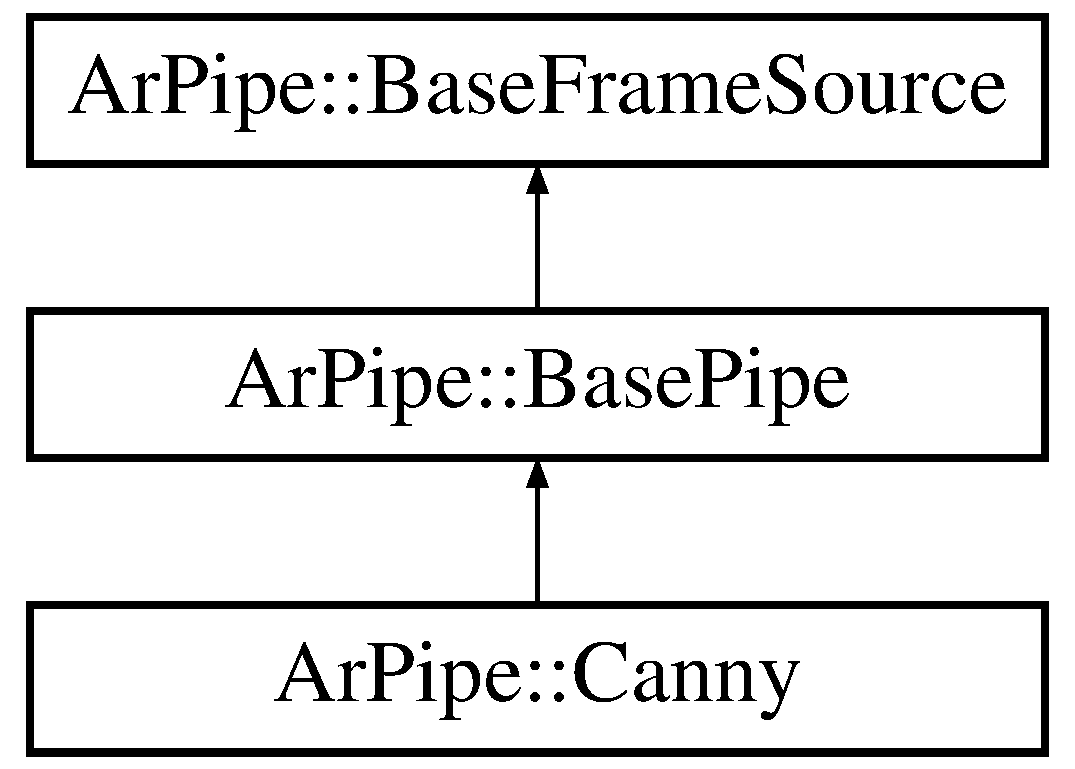
\includegraphics[height=3.000000cm]{d0/d36/class_ar_pipe_1_1_canny}
\end{center}
\end{figure}
\subsection*{Veřejné metody}
\begin{DoxyCompactItemize}
\item 
\hypertarget{class_ar_pipe_1_1_canny_aa806eb626a041a543c850b9755697717}{{\bfseries Canny} (\hyperlink{class_ar_pipe_1_1_base_frame_source}{Base\-Frame\-Source} $\ast$previous\-Pipe)}\label{d0/d36/class_ar_pipe_1_1_canny_aa806eb626a041a543c850b9755697717}

\item 
\hypertarget{class_ar_pipe_1_1_canny_a4579563ce17fcbfae02d4faa8a21ea64}{void {\bfseries process\-Frame\-Container} (\hyperlink{class_ar_pipe_1_1_base_frame_container}{Base\-Frame\-Container} $\ast$frm, \hyperlink{class_ar_pipe_1_1_base_frame_source}{Base\-Frame\-Source} $\ast$frame\-Source)}\label{d0/d36/class_ar_pipe_1_1_canny_a4579563ce17fcbfae02d4faa8a21ea64}

\item 
\hypertarget{class_ar_pipe_1_1_canny_ae515215ec103b8439489dde98aa11199}{\hyperlink{class_ar_pipe_1_1_canny}{Canny} $\ast$ {\bfseries set\-Thresholds} (double lower, double upper)}\label{d0/d36/class_ar_pipe_1_1_canny_ae515215ec103b8439489dde98aa11199}

\item 
\hypertarget{class_ar_pipe_1_1_canny_a7a2bd70d7401d8e8ca78ca6084d18ae2}{\hyperlink{class_ar_pipe_1_1_canny}{Canny} $\ast$ {\bfseries set\-Auto\-Threshold} ()}\label{d0/d36/class_ar_pipe_1_1_canny_a7a2bd70d7401d8e8ca78ca6084d18ae2}

\end{DoxyCompactItemize}
\subsection*{Statické veřejné metody}
\begin{DoxyCompactItemize}
\item 
\hypertarget{class_ar_pipe_1_1_canny_a0666e7fa073b18c16701b454d6d4ab03}{static \hyperlink{class_ar_pipe_1_1_canny}{Canny} $\ast$ {\bfseries init} ()}\label{d0/d36/class_ar_pipe_1_1_canny_a0666e7fa073b18c16701b454d6d4ab03}

\end{DoxyCompactItemize}
\subsection*{Chráněné metody}
\begin{DoxyCompactItemize}
\item 
\hypertarget{class_ar_pipe_1_1_canny_add40d70a37dce319f756ce68785020e4}{double {\bfseries get\-Lower\-Threshold} (\hyperlink{class_ar_pipe_1_1_frame}{Frame} $\ast$frm)}\label{d0/d36/class_ar_pipe_1_1_canny_add40d70a37dce319f756ce68785020e4}

\item 
\hypertarget{class_ar_pipe_1_1_canny_a9407db425e6ece4b3ba98d97cb705c9f}{double {\bfseries get\-Upper\-Threshold} (\hyperlink{class_ar_pipe_1_1_frame}{Frame} $\ast$frm)}\label{d0/d36/class_ar_pipe_1_1_canny_a9407db425e6ece4b3ba98d97cb705c9f}

\end{DoxyCompactItemize}
\subsection*{Chráněné atributy}
\begin{DoxyCompactItemize}
\item 
\hypertarget{class_ar_pipe_1_1_canny_a0df1206380fdaa984cebb3c333f548e7}{double {\bfseries lower\-Threshold}}\label{d0/d36/class_ar_pipe_1_1_canny_a0df1206380fdaa984cebb3c333f548e7}

\item 
\hypertarget{class_ar_pipe_1_1_canny_ac48771787a479f0dcb7269161da61099}{double {\bfseries upper\-Threshold}}\label{d0/d36/class_ar_pipe_1_1_canny_ac48771787a479f0dcb7269161da61099}

\item 
\hypertarget{class_ar_pipe_1_1_canny_a6d9cf95bbc2428326afce4aadcb993d8}{bool {\bfseries auto\-Thresholds}}\label{d0/d36/class_ar_pipe_1_1_canny_a6d9cf95bbc2428326afce4aadcb993d8}

\end{DoxyCompactItemize}


Dokumentace pro tuto třídu byla generována z následujících souborů\-:\begin{DoxyCompactItemize}
\item 
Pipes/\-Effects/Canny.\-h\item 
Pipes/\-Effects/Canny.\-cpp\end{DoxyCompactItemize}

\hypertarget{class_ar_pipe_1_1_detect_polygons}{\section{Dokumentace třídy Ar\-Pipe\-:\-:Detect\-Polygons}
\label{da/d76/class_ar_pipe_1_1_detect_polygons}\index{Ar\-Pipe\-::\-Detect\-Polygons@{Ar\-Pipe\-::\-Detect\-Polygons}}
}
Diagram dědičnosti pro třídu Ar\-Pipe\-:\-:Detect\-Polygons\begin{figure}[H]
\begin{center}
\leavevmode
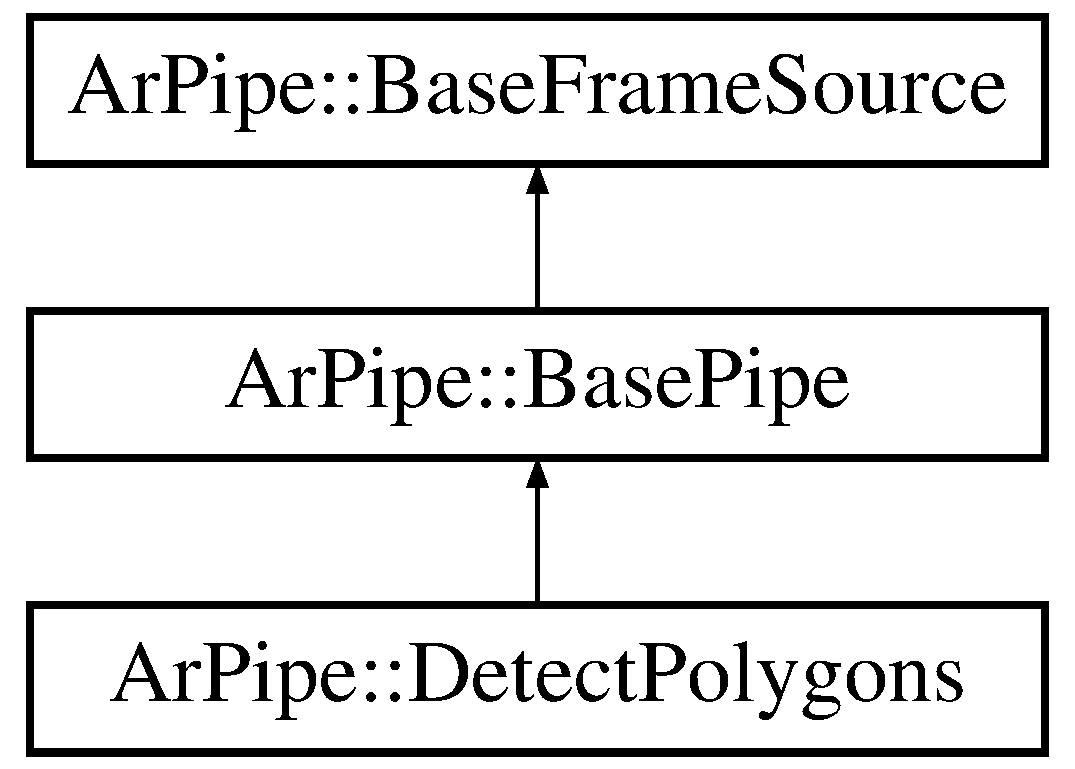
\includegraphics[height=3.000000cm]{da/d76/class_ar_pipe_1_1_detect_polygons}
\end{center}
\end{figure}
\subsection*{Veřejné metody}
\begin{DoxyCompactItemize}
\item 
\hypertarget{class_ar_pipe_1_1_detect_polygons_a132ddfcdd899cede29f93097b481e57e}{{\bfseries Detect\-Polygons} (\hyperlink{class_ar_pipe_1_1_base_frame_source}{Base\-Frame\-Source} $\ast$previous\-Pipe)}\label{da/d76/class_ar_pipe_1_1_detect_polygons_a132ddfcdd899cede29f93097b481e57e}

\item 
void \hyperlink{class_ar_pipe_1_1_detect_polygons_aac72d1077fe05672a2f6f2a33b960719}{process\-Frame\-Container} (\hyperlink{class_ar_pipe_1_1_base_frame_container}{Base\-Frame\-Container} $\ast$frm, \hyperlink{class_ar_pipe_1_1_base_frame_source}{Base\-Frame\-Source} $\ast$frame\-Source)
\item 
\hypertarget{class_ar_pipe_1_1_detect_polygons_a69ab6fede463ea15454feec13cdb56d4}{\hyperlink{class_ar_pipe_1_1_detect_polygons}{Detect\-Polygons} $\ast$ {\bfseries set\-Max\-Complexity} (int max=12)}\label{da/d76/class_ar_pipe_1_1_detect_polygons_a69ab6fede463ea15454feec13cdb56d4}

\item 
\hypertarget{class_ar_pipe_1_1_detect_polygons_a3d637f0ef505dd2b6aaf19e8477fd197}{\hyperlink{class_ar_pipe_1_1_detect_polygons}{Detect\-Polygons} $\ast$ {\bfseries set\-Min\-Complexity} (int min=2)}\label{da/d76/class_ar_pipe_1_1_detect_polygons_a3d637f0ef505dd2b6aaf19e8477fd197}

\item 
\hypertarget{class_ar_pipe_1_1_detect_polygons_af9d6a11e2cbd9dfbc003c87e25e425bc}{\hyperlink{class_ar_pipe_1_1_detect_polygons}{Detect\-Polygons} $\ast$ {\bfseries set\-Min\-Distance} (int distance=0)}\label{da/d76/class_ar_pipe_1_1_detect_polygons_af9d6a11e2cbd9dfbc003c87e25e425bc}

\item 
\hypertarget{class_ar_pipe_1_1_detect_polygons_ac7c8e88f1f23987bd138555475cb158e}{\hyperlink{class_ar_pipe_1_1_detect_polygons}{Detect\-Polygons} $\ast$ {\bfseries set\-Complexity\-Koef} (float koef=0.\-05)}\label{da/d76/class_ar_pipe_1_1_detect_polygons_ac7c8e88f1f23987bd138555475cb158e}

\item 
\hypertarget{class_ar_pipe_1_1_detect_polygons_a891e5579b3c0e500e1daad42501394ad}{\hyperlink{class_ar_pipe_1_1_detect_polygons}{Detect\-Polygons} $\ast$ {\bfseries set\-Straighten\-Lines} (bool straighten=true)}\label{da/d76/class_ar_pipe_1_1_detect_polygons_a891e5579b3c0e500e1daad42501394ad}

\item 
\hypertarget{class_ar_pipe_1_1_detect_polygons_a3e73ca1de8c73f0d3b7ffee515ca326f}{\hyperlink{class_ar_pipe_1_1_detect_polygons}{Detect\-Polygons} $\ast$ {\bfseries set\-Minimal\-Sides} (unsigned int sides=4)}\label{da/d76/class_ar_pipe_1_1_detect_polygons_a3e73ca1de8c73f0d3b7ffee515ca326f}

\item 
\hypertarget{class_ar_pipe_1_1_detect_polygons_a3ab5ade150b5688bf4e1623c35da8b8e}{\hyperlink{class_ar_pipe_1_1_detect_polygons}{Detect\-Polygons} $\ast$ {\bfseries set\-Maximal\-Sides} (unsigned int sides=I\-N\-T\-\_\-\-M\-A\-X)}\label{da/d76/class_ar_pipe_1_1_detect_polygons_a3ab5ade150b5688bf4e1623c35da8b8e}

\item 
\hypertarget{class_ar_pipe_1_1_detect_polygons_acfe20948b75391eb94e9ee36afb1ee40}{\hyperlink{class_ar_pipe_1_1_detect_polygons}{Detect\-Polygons} $\ast$ {\bfseries set\-Required\-Side\-Count} (unsigned int sides)}\label{da/d76/class_ar_pipe_1_1_detect_polygons_acfe20948b75391eb94e9ee36afb1ee40}

\item 
\hypertarget{class_ar_pipe_1_1_detect_polygons_aec7c48f8a867b3f614b28df69e40315b}{\hyperlink{class_ar_pipe_1_1_detect_polygons}{Detect\-Polygons} $\ast$ {\bfseries set\-Only\-Convex\-Objects} (bool convex=true)}\label{da/d76/class_ar_pipe_1_1_detect_polygons_aec7c48f8a867b3f614b28df69e40315b}

\item 
\hypertarget{class_ar_pipe_1_1_detect_polygons_aabb95232ff4714056785cf6f437a7d4f}{\hyperlink{class_ar_pipe_1_1_detect_polygons}{Detect\-Polygons} $\ast$ {\bfseries set\-Need\-Closed\-Objects} (bool closed=true)}\label{da/d76/class_ar_pipe_1_1_detect_polygons_aabb95232ff4714056785cf6f437a7d4f}

\end{DoxyCompactItemize}
\subsection*{Statické veřejné metody}
\begin{DoxyCompactItemize}
\item 
\hypertarget{class_ar_pipe_1_1_detect_polygons_acc4d465f718feca3ba1a25738aaed06a}{static \hyperlink{class_ar_pipe_1_1_detect_polygons}{Detect\-Polygons} $\ast$ {\bfseries init} ()}\label{da/d76/class_ar_pipe_1_1_detect_polygons_acc4d465f718feca3ba1a25738aaed06a}

\end{DoxyCompactItemize}
\subsection*{Chráněné metody}
\begin{DoxyCompactItemize}
\item 
\hypertarget{class_ar_pipe_1_1_detect_polygons_a3b632b18d174e706cdffdd8ae16187fb}{int {\bfseries perimeter} (std\-::vector$<$ cv\-::\-Point2f $>$ \&a)}\label{da/d76/class_ar_pipe_1_1_detect_polygons_a3b632b18d174e706cdffdd8ae16187fb}

\item 
{\footnotesize template$<$typename T $>$ }\\void \hyperlink{class_ar_pipe_1_1_detect_polygons_a5027e25c5bdc3ab0e70f3d4a6c47369d}{remove\-Elements} (std\-::vector$<$ T $>$ \&vinout, const std\-::vector$<$ bool $>$ \&to\-Remove)
\end{DoxyCompactItemize}
\subsection*{Chráněné atributy}
\begin{DoxyCompactItemize}
\item 
\hypertarget{class_ar_pipe_1_1_detect_polygons_aa05d1826c1375141a3bae4c076c33782}{int {\bfseries max\-Complexity}}\label{da/d76/class_ar_pipe_1_1_detect_polygons_aa05d1826c1375141a3bae4c076c33782}

\item 
\hypertarget{class_ar_pipe_1_1_detect_polygons_a4e1dd06724dad6cfa4d47055a0bb687e}{int {\bfseries min\-Complexity}}\label{da/d76/class_ar_pipe_1_1_detect_polygons_a4e1dd06724dad6cfa4d47055a0bb687e}

\item 
\hypertarget{class_ar_pipe_1_1_detect_polygons_a9bef113248ad45b7ad282d9c4389c6d2}{int {\bfseries min\-Distance}}\label{da/d76/class_ar_pipe_1_1_detect_polygons_a9bef113248ad45b7ad282d9c4389c6d2}

\item 
\hypertarget{class_ar_pipe_1_1_detect_polygons_a93b51a66554399f5d06fad49f06d038c}{float {\bfseries complexity\-Koef}}\label{da/d76/class_ar_pipe_1_1_detect_polygons_a93b51a66554399f5d06fad49f06d038c}

\item 
\hypertarget{class_ar_pipe_1_1_detect_polygons_ac1da91b5f863368e028a0d8f1dc9df7d}{bool {\bfseries simplify\-Polygons}}\label{da/d76/class_ar_pipe_1_1_detect_polygons_ac1da91b5f863368e028a0d8f1dc9df7d}

\item 
\hypertarget{class_ar_pipe_1_1_detect_polygons_a4990e15bc56381ea1deec7dcb21ce8d2}{unsigned int {\bfseries minimal\-Polygon\-Lines}}\label{da/d76/class_ar_pipe_1_1_detect_polygons_a4990e15bc56381ea1deec7dcb21ce8d2}

\item 
\hypertarget{class_ar_pipe_1_1_detect_polygons_ab052508f83ccab2ed0ed15c76a91b766}{unsigned int {\bfseries maximal\-Polygon\-Lines}}\label{da/d76/class_ar_pipe_1_1_detect_polygons_ab052508f83ccab2ed0ed15c76a91b766}

\item 
\hypertarget{class_ar_pipe_1_1_detect_polygons_acb497e785444095892d6d0e355ab9b60}{bool {\bfseries only\-Convex}}\label{da/d76/class_ar_pipe_1_1_detect_polygons_acb497e785444095892d6d0e355ab9b60}

\item 
\hypertarget{class_ar_pipe_1_1_detect_polygons_a8e9e725c801856beeb3ee7703b804c4f}{bool {\bfseries only\-Closed}}\label{da/d76/class_ar_pipe_1_1_detect_polygons_a8e9e725c801856beeb3ee7703b804c4f}

\end{DoxyCompactItemize}


\subsection{Dokumentace k metodám}
\hypertarget{class_ar_pipe_1_1_detect_polygons_aac72d1077fe05672a2f6f2a33b960719}{\index{Ar\-Pipe\-::\-Detect\-Polygons@{Ar\-Pipe\-::\-Detect\-Polygons}!process\-Frame\-Container@{process\-Frame\-Container}}
\index{process\-Frame\-Container@{process\-Frame\-Container}!ArPipe::DetectPolygons@{Ar\-Pipe\-::\-Detect\-Polygons}}
\subsubsection[{process\-Frame\-Container}]{\setlength{\rightskip}{0pt plus 5cm}void Ar\-Pipe\-::\-Detect\-Polygons\-::process\-Frame\-Container (
\begin{DoxyParamCaption}
\item[{{\bf Base\-Frame\-Container} $\ast$}]{frm, }
\item[{{\bf Base\-Frame\-Source} $\ast$}]{frame\-Source}
\end{DoxyParamCaption}
)\hspace{0.3cm}{\ttfamily [virtual]}}}\label{da/d76/class_ar_pipe_1_1_detect_polygons_aac72d1077fe05672a2f6f2a33b960719}
for each contour, analyze if it is a paralelepiped likely to be the marker

remove these elements whise corners are too close to each other 

Reimplementuje stejnojmenný prvek z \hyperlink{class_ar_pipe_1_1_base_pipe}{Ar\-Pipe\-::\-Base\-Pipe}.

\hypertarget{class_ar_pipe_1_1_detect_polygons_a5027e25c5bdc3ab0e70f3d4a6c47369d}{\index{Ar\-Pipe\-::\-Detect\-Polygons@{Ar\-Pipe\-::\-Detect\-Polygons}!remove\-Elements@{remove\-Elements}}
\index{remove\-Elements@{remove\-Elements}!ArPipe::DetectPolygons@{Ar\-Pipe\-::\-Detect\-Polygons}}
\subsubsection[{remove\-Elements}]{\setlength{\rightskip}{0pt plus 5cm}template$<$typename T $>$ void Ar\-Pipe\-::\-Detect\-Polygons\-::remove\-Elements (
\begin{DoxyParamCaption}
\item[{std\-::vector$<$ T $>$ \&}]{vinout, }
\item[{const std\-::vector$<$ bool $>$ \&}]{to\-Remove}
\end{DoxyParamCaption}
)\hspace{0.3cm}{\ttfamily [protected]}}}\label{da/d76/class_ar_pipe_1_1_detect_polygons_a5027e25c5bdc3ab0e70f3d4a6c47369d}
Given a vector vinout with elements and a boolean vector indicating the lements from it to remove, this function remove the elements 
\begin{DoxyParams}{Parametry}
{\em vinout} & \\
\hline
{\em to\-Remove} & \\
\hline
\end{DoxyParams}


Dokumentace pro tuto třídu byla generována z následujících souborů\-:\begin{DoxyCompactItemize}
\item 
Pipes/\-Recognizers/Detect\-Polygons.\-h\item 
Pipes/\-Recognizers/Detect\-Polygons.\-cpp\end{DoxyCompactItemize}

\hypertarget{class_ar_pipe_1_1_draw_contours}{\section{Dokumentace třídy Ar\-Pipe\-:\-:Draw\-Contours}
\label{db/d85/class_ar_pipe_1_1_draw_contours}\index{Ar\-Pipe\-::\-Draw\-Contours@{Ar\-Pipe\-::\-Draw\-Contours}}
}
Diagram dědičnosti pro třídu Ar\-Pipe\-:\-:Draw\-Contours\begin{figure}[H]
\begin{center}
\leavevmode
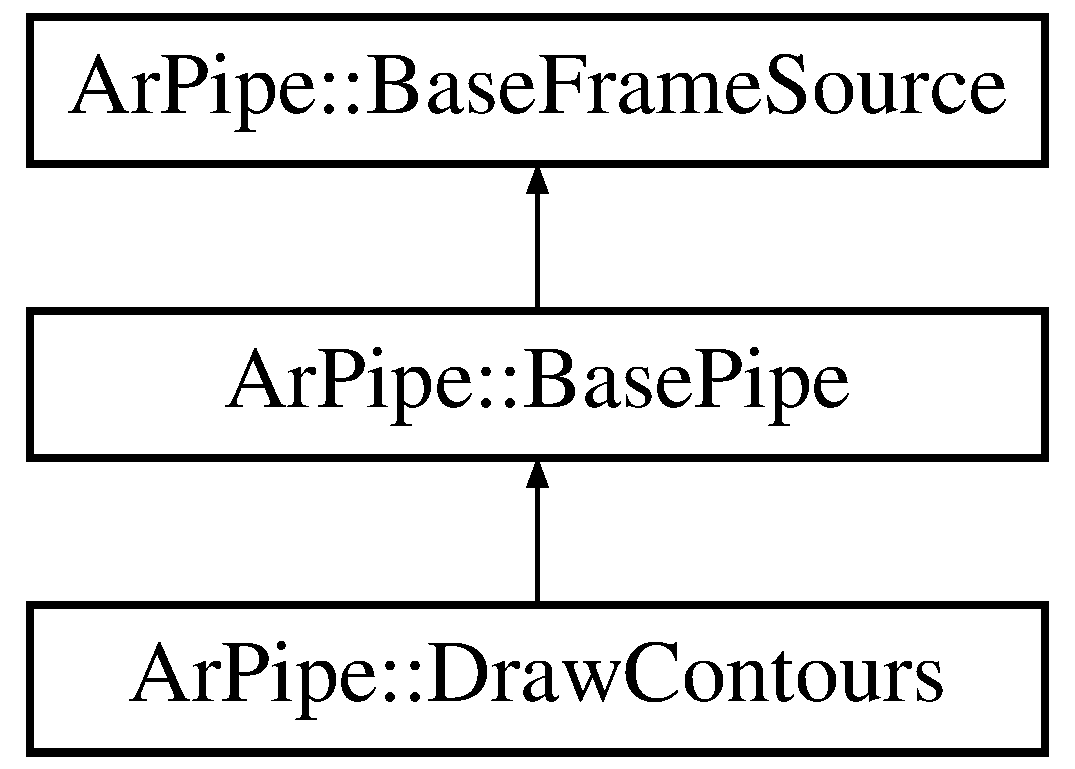
\includegraphics[height=3.000000cm]{db/d85/class_ar_pipe_1_1_draw_contours}
\end{center}
\end{figure}
\subsection*{Veřejné metody}
\begin{DoxyCompactItemize}
\item 
\hypertarget{class_ar_pipe_1_1_draw_contours_aa6eaef1d9ee0e61b0b4424f28e5bea37}{{\bfseries Draw\-Contours} (\hyperlink{class_ar_pipe_1_1_base_frame_source}{Base\-Frame\-Source} $\ast$previous\-Pipe)}\label{db/d85/class_ar_pipe_1_1_draw_contours_aa6eaef1d9ee0e61b0b4424f28e5bea37}

\item 
\hypertarget{class_ar_pipe_1_1_draw_contours_abcf5ab4fb2e7e9d7fbecbe84e2fe6f1c}{void {\bfseries process\-Frame\-Container} (\hyperlink{class_ar_pipe_1_1_base_frame_container}{Base\-Frame\-Container} $\ast$frm, \hyperlink{class_ar_pipe_1_1_base_frame_source}{Base\-Frame\-Source} $\ast$frame\-Source)}\label{db/d85/class_ar_pipe_1_1_draw_contours_abcf5ab4fb2e7e9d7fbecbe84e2fe6f1c}

\end{DoxyCompactItemize}
\subsection*{Statické veřejné metody}
\begin{DoxyCompactItemize}
\item 
\hypertarget{class_ar_pipe_1_1_draw_contours_a5ca78f9cbefc9f7bf8dbeb95f53fe870}{static \hyperlink{class_ar_pipe_1_1_draw_contours}{Draw\-Contours} $\ast$ {\bfseries init} ()}\label{db/d85/class_ar_pipe_1_1_draw_contours_a5ca78f9cbefc9f7bf8dbeb95f53fe870}

\end{DoxyCompactItemize}
\subsection*{Chráněné atributy}
\begin{DoxyCompactItemize}
\item 
\hypertarget{class_ar_pipe_1_1_draw_contours_a5d0e5819dcc6c7ba0ee109d40e526939}{int {\bfseries thickness}}\label{db/d85/class_ar_pipe_1_1_draw_contours_a5d0e5819dcc6c7ba0ee109d40e526939}

\item 
\hypertarget{class_ar_pipe_1_1_draw_contours_accb67a77f3281177187bb7f360c22e3d}{int {\bfseries line\-Type}}\label{db/d85/class_ar_pipe_1_1_draw_contours_accb67a77f3281177187bb7f360c22e3d}

\item 
\hypertarget{class_ar_pipe_1_1_draw_contours_a123fcf80721b18f66a15923d01458f04}{int {\bfseries max\-Level}}\label{db/d85/class_ar_pipe_1_1_draw_contours_a123fcf80721b18f66a15923d01458f04}

\item 
\hypertarget{class_ar_pipe_1_1_draw_contours_adeb714c56926f49e3de3e519c7b3e484}{cv\-::\-Scalar {\bfseries color}}\label{db/d85/class_ar_pipe_1_1_draw_contours_adeb714c56926f49e3de3e519c7b3e484}

\end{DoxyCompactItemize}


Dokumentace pro tuto třídu byla generována z následujících souborů\-:\begin{DoxyCompactItemize}
\item 
Pipes/\-Drawers/Draw\-Contrours.\-h\item 
Pipes/\-Drawers/Draw\-Contrours.\-cpp\end{DoxyCompactItemize}

\hypertarget{class_ar_pipe_1_1_find_contours}{\section{Dokumentace třídy Ar\-Pipe\-:\-:Find\-Contours}
\label{db/db3/class_ar_pipe_1_1_find_contours}\index{Ar\-Pipe\-::\-Find\-Contours@{Ar\-Pipe\-::\-Find\-Contours}}
}
Diagram dědičnosti pro třídu Ar\-Pipe\-:\-:Find\-Contours\begin{figure}[H]
\begin{center}
\leavevmode
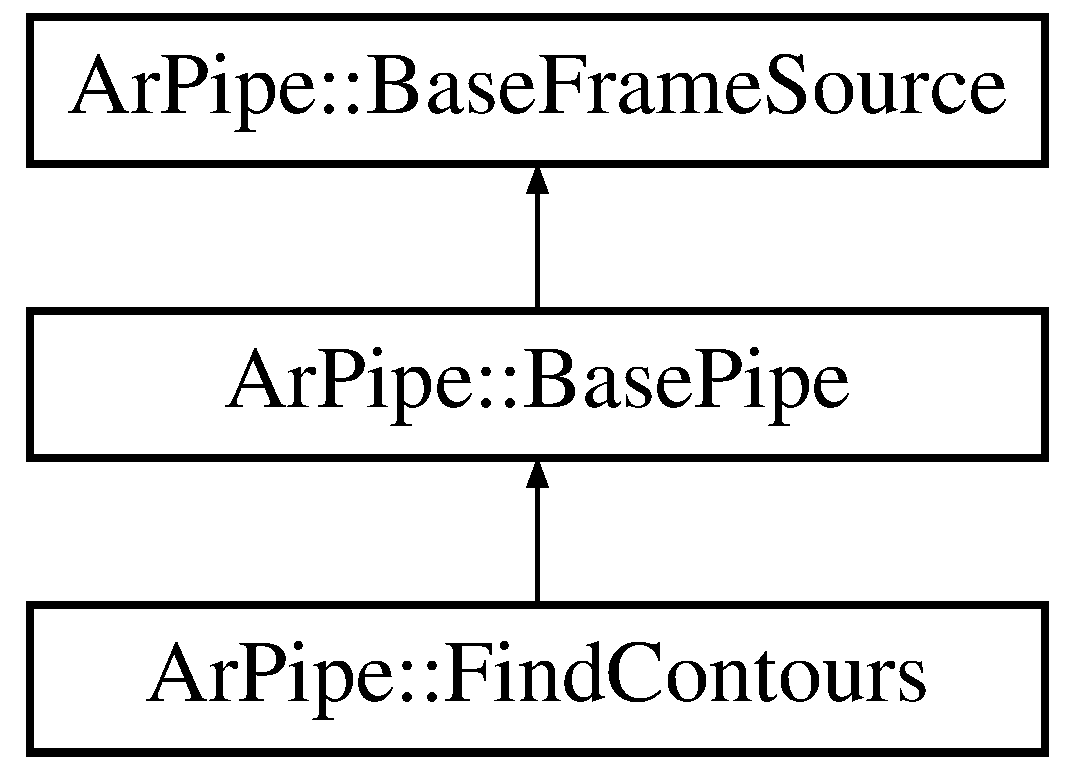
\includegraphics[height=3.000000cm]{db/db3/class_ar_pipe_1_1_find_contours}
\end{center}
\end{figure}
\subsection*{Veřejné metody}
\begin{DoxyCompactItemize}
\item 
\hypertarget{class_ar_pipe_1_1_find_contours_a45d7cdb88cead31995663199a40bd865}{{\bfseries Find\-Contours} (\hyperlink{class_ar_pipe_1_1_base_frame_source}{Base\-Frame\-Source} $\ast$previous\-Pipe)}\label{db/db3/class_ar_pipe_1_1_find_contours_a45d7cdb88cead31995663199a40bd865}

\item 
\hypertarget{class_ar_pipe_1_1_find_contours_aa014521127836032f288a49e00f88f87}{void {\bfseries process\-Frame\-Container} (\hyperlink{class_ar_pipe_1_1_base_frame_container}{Base\-Frame\-Container} $\ast$frm, \hyperlink{class_ar_pipe_1_1_base_frame_source}{Base\-Frame\-Source} $\ast$frame\-Source)}\label{db/db3/class_ar_pipe_1_1_find_contours_aa014521127836032f288a49e00f88f87}

\item 
\hypertarget{class_ar_pipe_1_1_find_contours_a82244ef64d0f31acbcec69edc00ec44e}{\hyperlink{class_ar_pipe_1_1_find_contours}{Find\-Contours} $\ast$ {\bfseries set\-Type\-Only\-External} ()}\label{db/db3/class_ar_pipe_1_1_find_contours_a82244ef64d0f31acbcec69edc00ec44e}

\item 
\hypertarget{class_ar_pipe_1_1_find_contours_a81c631d105161494348fb9645a57d39b}{\hyperlink{class_ar_pipe_1_1_find_contours}{Find\-Contours} $\ast$ {\bfseries set\-Type\-List} ()}\label{db/db3/class_ar_pipe_1_1_find_contours_a81c631d105161494348fb9645a57d39b}

\item 
\hypertarget{class_ar_pipe_1_1_find_contours_aadfcfc69eadfb8ac6285c6c8e2d71858}{\hyperlink{class_ar_pipe_1_1_find_contours}{Find\-Contours} $\ast$ {\bfseries set\-Type\-Tree} ()}\label{db/db3/class_ar_pipe_1_1_find_contours_aadfcfc69eadfb8ac6285c6c8e2d71858}

\item 
\hypertarget{class_ar_pipe_1_1_find_contours_a429e0aa3153b67a9eff7ec9444cf6c4b}{\hyperlink{class_ar_pipe_1_1_find_contours}{Find\-Contours} $\ast$ {\bfseries set\-C\-Comp} ()}\label{db/db3/class_ar_pipe_1_1_find_contours_a429e0aa3153b67a9eff7ec9444cf6c4b}

\item 
\hypertarget{class_ar_pipe_1_1_find_contours_a8ef65dd34799927f6c4130fdee0327a6}{\hyperlink{class_ar_pipe_1_1_find_contours}{Find\-Contours} $\ast$ {\bfseries set\-Aprox\-None} ()}\label{db/db3/class_ar_pipe_1_1_find_contours_a8ef65dd34799927f6c4130fdee0327a6}

\item 
\hypertarget{class_ar_pipe_1_1_find_contours_a0f81507b31a6128432c1d15c6055c413}{\hyperlink{class_ar_pipe_1_1_find_contours}{Find\-Contours} $\ast$ {\bfseries set\-Aprox\-Tc} (bool kcos)}\label{db/db3/class_ar_pipe_1_1_find_contours_a0f81507b31a6128432c1d15c6055c413}

\end{DoxyCompactItemize}
\subsection*{Statické veřejné metody}
\begin{DoxyCompactItemize}
\item 
\hypertarget{class_ar_pipe_1_1_find_contours_a4b9c20aaf857866d9559d33edaf57a82}{static \hyperlink{class_ar_pipe_1_1_find_contours}{Find\-Contours} $\ast$ {\bfseries init} ()}\label{db/db3/class_ar_pipe_1_1_find_contours_a4b9c20aaf857866d9559d33edaf57a82}

\end{DoxyCompactItemize}
\subsection*{Chráněné atributy}
\begin{DoxyCompactItemize}
\item 
\hypertarget{class_ar_pipe_1_1_find_contours_a50a3f91071bc9b8650817b3b55bdc154}{int {\bfseries mode}}\label{db/db3/class_ar_pipe_1_1_find_contours_a50a3f91071bc9b8650817b3b55bdc154}

\item 
\hypertarget{class_ar_pipe_1_1_find_contours_a5c4eccb58ea37953f12850110228dc53}{int {\bfseries method}}\label{db/db3/class_ar_pipe_1_1_find_contours_a5c4eccb58ea37953f12850110228dc53}

\end{DoxyCompactItemize}


Dokumentace pro tuto třídu byla generována z následujících souborů\-:\begin{DoxyCompactItemize}
\item 
Pipes/\-Recognizers/Find\-Contours.\-h\item 
Pipes/\-Recognizers/Find\-Contours.\-cpp\end{DoxyCompactItemize}

\hypertarget{class_ar_pipe_1_1_frame}{\section{Dokumentace třídy Ar\-Pipe\-:\-:Frame}
\label{dd/d9d/class_ar_pipe_1_1_frame}\index{Ar\-Pipe\-::\-Frame@{Ar\-Pipe\-::\-Frame}}
}
\subsection*{Veřejné metody}
\begin{DoxyCompactItemize}
\item 
\hypertarget{class_ar_pipe_1_1_frame_a7df86733519e85d78810c42e3af6d705}{{\bfseries Frame} (Mat frm)}\label{dd/d9d/class_ar_pipe_1_1_frame_a7df86733519e85d78810c42e3af6d705}

\item 
\hypertarget{class_ar_pipe_1_1_frame_afa0519f1ec506df02dfdce31bc5f60b0}{\hyperlink{class_ar_pipe_1_1_frame}{Frame} $\ast$ {\bfseries clone} ()}\label{dd/d9d/class_ar_pipe_1_1_frame_afa0519f1ec506df02dfdce31bc5f60b0}

\item 
\hypertarget{class_ar_pipe_1_1_frame_a288d704c6ca113753dc2f475ebba7060}{Mat \& {\bfseries get\-Mat} ()}\label{dd/d9d/class_ar_pipe_1_1_frame_a288d704c6ca113753dc2f475ebba7060}

\item 
\hypertarget{class_ar_pipe_1_1_frame_a280244b050dd0d620de5c32f7e061636}{void {\bfseries rotate} (int degrees)}\label{dd/d9d/class_ar_pipe_1_1_frame_a280244b050dd0d620de5c32f7e061636}

\item 
\hypertarget{class_ar_pipe_1_1_frame_a07610312b8cf3a3ed93f110bb79af65b}{bool {\bfseries is\-Grey} ()}\label{dd/d9d/class_ar_pipe_1_1_frame_a07610312b8cf3a3ed93f110bb79af65b}

\item 
\hypertarget{class_ar_pipe_1_1_frame_a027366e8e62fb46c7bf417588f7b5fe0}{int {\bfseries get\-Channel\-Count} ()}\label{dd/d9d/class_ar_pipe_1_1_frame_a027366e8e62fb46c7bf417588f7b5fe0}

\item 
double \hyperlink{class_ar_pipe_1_1_frame_a943c88c01272f29a6fde81deb045e63f}{get\-Depth} ()
\end{DoxyCompactItemize}
\subsection*{Veřejné atributy}
\begin{DoxyCompactItemize}
\item 
\hypertarget{class_ar_pipe_1_1_frame_afa105fc13822a413d8202c386376c2f2}{Mat {\bfseries frame}}\label{dd/d9d/class_ar_pipe_1_1_frame_afa105fc13822a413d8202c386376c2f2}

\end{DoxyCompactItemize}


\subsection{Dokumentace k metodám}
\hypertarget{class_ar_pipe_1_1_frame_a943c88c01272f29a6fde81deb045e63f}{\index{Ar\-Pipe\-::\-Frame@{Ar\-Pipe\-::\-Frame}!get\-Depth@{get\-Depth}}
\index{get\-Depth@{get\-Depth}!ArPipe::Frame@{Ar\-Pipe\-::\-Frame}}
\subsubsection[{get\-Depth}]{\setlength{\rightskip}{0pt plus 5cm}double Ar\-Pipe\-::\-Frame\-::get\-Depth (
\begin{DoxyParamCaption}
{}
\end{DoxyParamCaption}
)}}\label{dd/d9d/class_ar_pipe_1_1_frame_a943c88c01272f29a6fde81deb045e63f}
C\-V\-\_\-8\-U -\/ 8-\/bit unsigned integers ( 0..255 ) C\-V\-\_\-8\-S -\/ 8-\/bit signed integers ( -\/128..127 ) C\-V\-\_\-16\-U -\/ 16-\/bit unsigned integers ( 0..65535 ) C\-V\-\_\-16\-S -\/ 16-\/bit signed integers ( -\/32768..32767 ) C\-V\-\_\-32\-S -\/ 32-\/bit signed integers ( -\/2147483648..2147483647 ) C\-V\-\_\-32\-F -\/ 32-\/bit floating-\/point numbers ( -\/\-F\-L\-T\-\_\-\-M\-A\-X..F\-L\-T\-\_\-\-M\-A\-X, I\-N\-F, N\-A\-N ) C\-V\-\_\-64\-F -\/ 64-\/bit floating-\/point numbers ( -\/\-D\-B\-L\-\_\-\-M\-A\-X..D\-B\-L\-\_\-\-M\-A\-X, I\-N\-F, N\-A\-N )

Dokumentace pro tuto třídu byla generována z následujících souborů\-:\begin{DoxyCompactItemize}
\item 
Model/Frame.\-h\item 
Model/Frame.\-cpp\end{DoxyCompactItemize}

\hypertarget{interface_g_l_renderer}{\section{Dokumentace třídy G\-L\-Renderer}
\label{d5/d74/interface_g_l_renderer}\index{G\-L\-Renderer@{G\-L\-Renderer}}
}
Diagram dědičnosti pro třídu G\-L\-Renderer\begin{figure}[H]
\begin{center}
\leavevmode
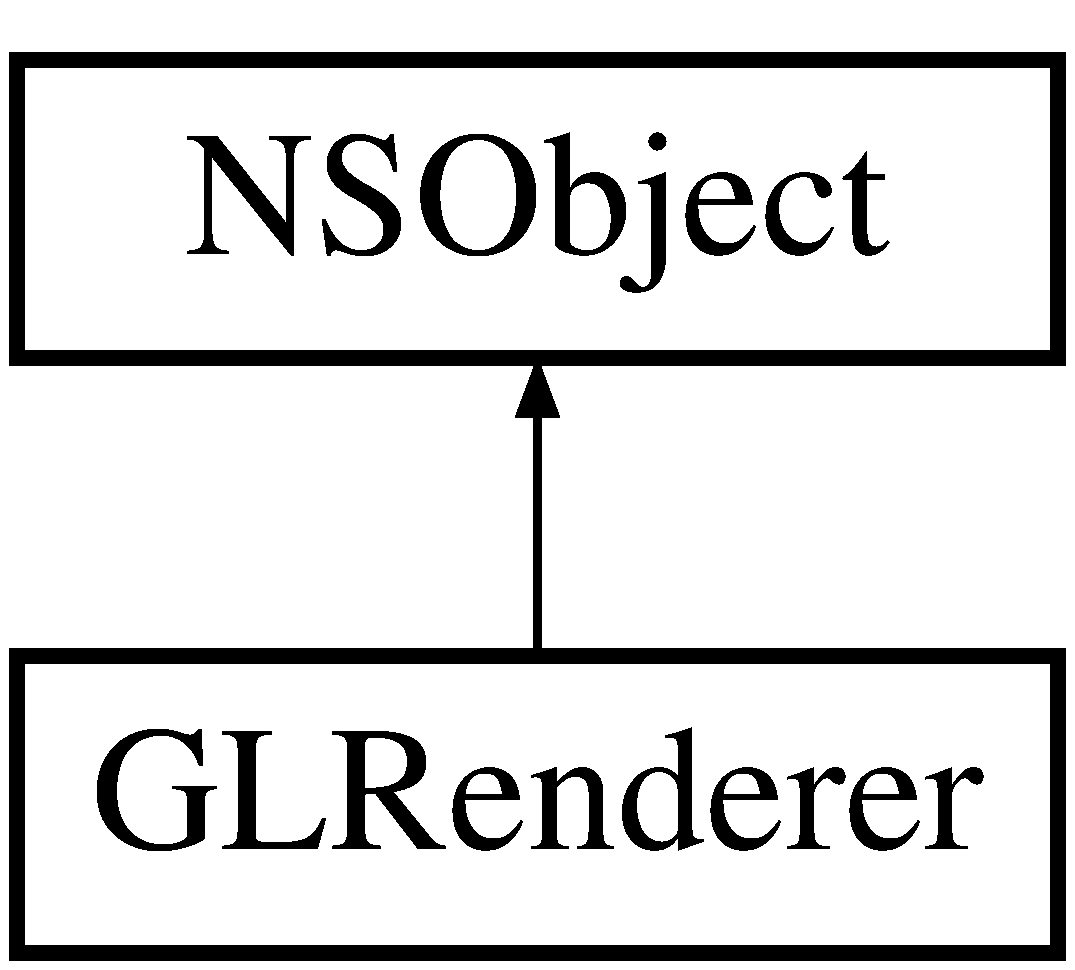
\includegraphics[height=2.000000cm]{d5/d74/interface_g_l_renderer}
\end{center}
\end{figure}
\subsection*{Metody instance}
\begin{DoxyCompactItemize}
\item 
\hypertarget{interface_g_l_renderer_a11f59d33b52e372234722f8353fcc69a}{(void) -\/ {\bfseries render}}\label{d5/d74/interface_g_l_renderer_a11f59d33b52e372234722f8353fcc69a}

\item 
\hypertarget{interface_g_l_renderer_ae10201bbf81b7881d8fdc2a37c701abf}{(B\-O\-O\-L) -\/ {\bfseries resize\-From\-Layer\-:}}\label{d5/d74/interface_g_l_renderer_ae10201bbf81b7881d8fdc2a37c701abf}

\item 
\hypertarget{interface_g_l_renderer_a57f9575f5f2bf14f62f80e48183b77f9}{(void) -\/ {\bfseries set\-Projection\-Matrix\-:}}\label{d5/d74/interface_g_l_renderer_a57f9575f5f2bf14f62f80e48183b77f9}

\item 
\hypertarget{interface_g_l_renderer_a526213b60809cc66a718cb8cf131a99f}{(void) -\/ {\bfseries set\-Model\-View\-Matrix\-:}}\label{d5/d74/interface_g_l_renderer_a526213b60809cc66a718cb8cf131a99f}

\end{DoxyCompactItemize}


Dokumentace pro tuto třídu byla generována z následujících souborů\-:\begin{DoxyCompactItemize}
\item 
U\-I/G\-L\-Renderer.\-h\item 
U\-I/G\-L\-Renderer.\-m\end{DoxyCompactItemize}

\hypertarget{interface_g_l_view}{\section{Dokumentace třídy G\-L\-View}
\label{d8/d4d/interface_g_l_view}\index{G\-L\-View@{G\-L\-View}}
}
Diagram dědičnosti pro třídu G\-L\-View\begin{figure}[H]
\begin{center}
\leavevmode
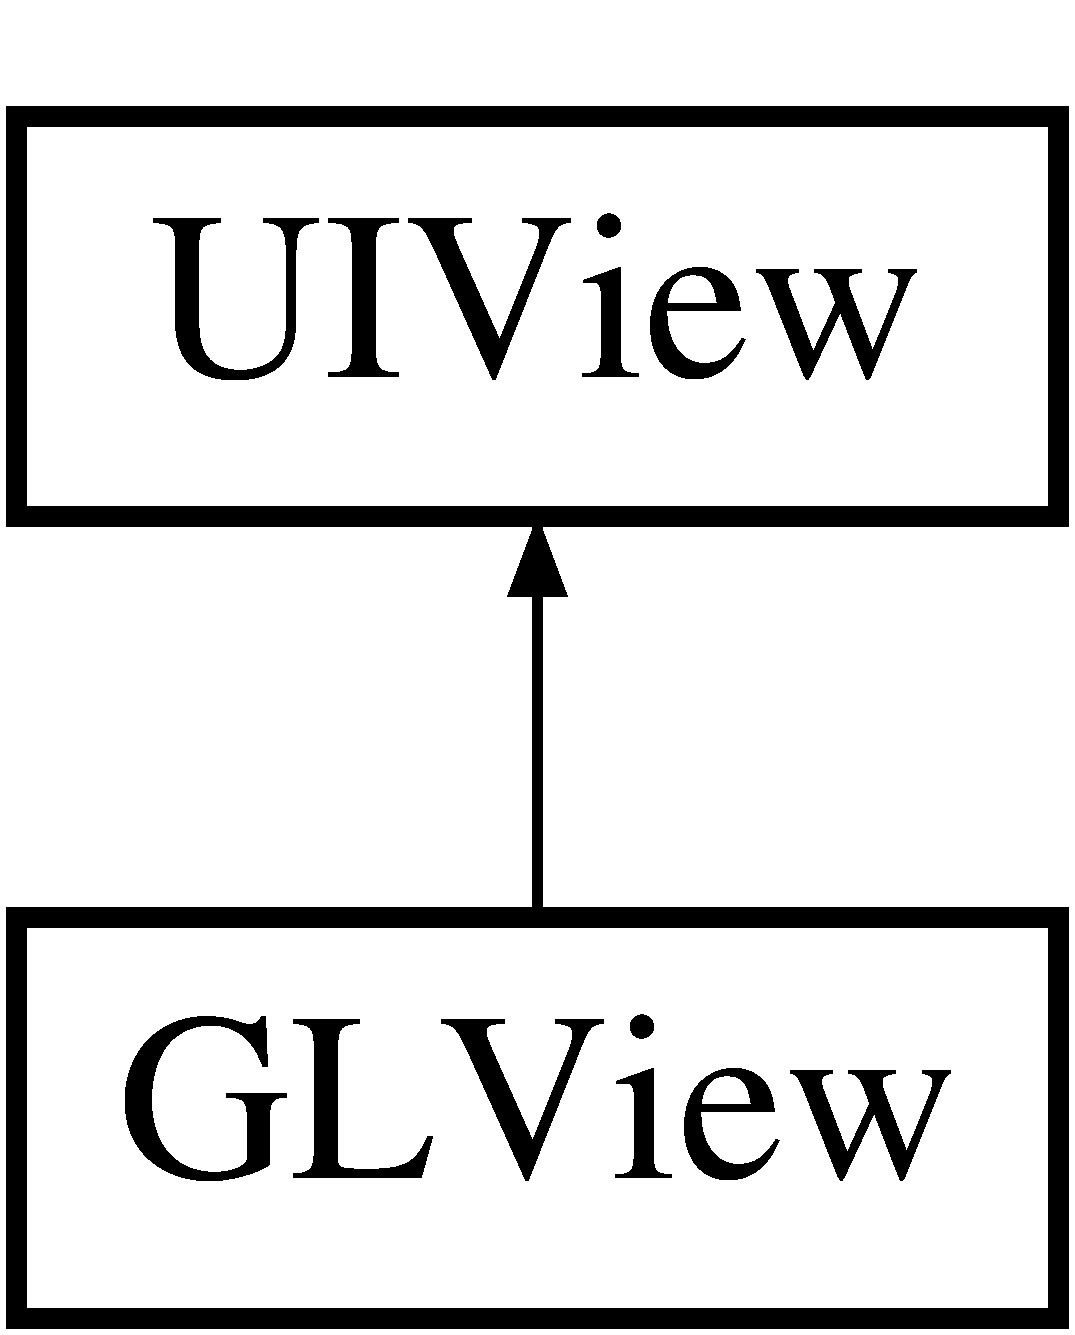
\includegraphics[height=2.000000cm]{d8/d4d/interface_g_l_view}
\end{center}
\end{figure}
\subsection*{Metody instance}
\begin{DoxyCompactItemize}
\item 
\hypertarget{interface_g_l_view_a22d6451905d60e51e3e23a486a2243de}{(void) -\/ {\bfseries start\-Animation}}\label{d8/d4d/interface_g_l_view_a22d6451905d60e51e3e23a486a2243de}

\item 
\hypertarget{interface_g_l_view_ad37cc85d6212e293a99201d109290411}{(void) -\/ {\bfseries stop\-Animation}}\label{d8/d4d/interface_g_l_view_ad37cc85d6212e293a99201d109290411}

\item 
\hypertarget{interface_g_l_view_a8d86e3e84cafd72716c4bbec79011ccc}{(void) -\/ {\bfseries draw\-View\-:}}\label{d8/d4d/interface_g_l_view_a8d86e3e84cafd72716c4bbec79011ccc}

\item 
\hypertarget{interface_g_l_view_adf40e47ba4b2e100ae12b9e0b6f54f9a}{(void) -\/ {\bfseries set\-Projection\-Matrix\-:}}\label{d8/d4d/interface_g_l_view_adf40e47ba4b2e100ae12b9e0b6f54f9a}

\item 
\hypertarget{interface_g_l_view_a43df1d959c1218d0a37b47bfd5dc6395}{(void) -\/ {\bfseries set\-Model\-View\-Matrix\-:}}\label{d8/d4d/interface_g_l_view_a43df1d959c1218d0a37b47bfd5dc6395}

\end{DoxyCompactItemize}
\subsection*{Vlastnosti}
\begin{DoxyCompactItemize}
\item 
\hypertarget{interface_g_l_view_ab42d23036c1353fe406be903c4cb2444}{B\-O\-O\-L {\bfseries animating}}\label{d8/d4d/interface_g_l_view_ab42d23036c1353fe406be903c4cb2444}

\item 
\hypertarget{interface_g_l_view_a379acc432018d6a4c2685d84a66e3ab9}{N\-S\-Integer {\bfseries animation\-Frame\-Interval}}\label{d8/d4d/interface_g_l_view_a379acc432018d6a4c2685d84a66e3ab9}

\end{DoxyCompactItemize}


Dokumentace pro tuto třídu byla generována z následujících souborů\-:\begin{DoxyCompactItemize}
\item 
U\-I/G\-L\-View.\-h\item 
U\-I/G\-L\-View.\-m\end{DoxyCompactItemize}

\hypertarget{class_ar_pipe_1_1_marker}{\section{Dokumentace třídy Ar\-Pipe\-:\-:Marker}
\label{d4/dc2/class_ar_pipe_1_1_marker}\index{Ar\-Pipe\-::\-Marker@{Ar\-Pipe\-::\-Marker}}
}


This class represents a marker. It is a vector of the fours corners ot the marker.  




{\ttfamily \#include $<$Marker.\-h$>$}

Diagram dědičnosti pro třídu Ar\-Pipe\-:\-:Marker\begin{figure}[H]
\begin{center}
\leavevmode
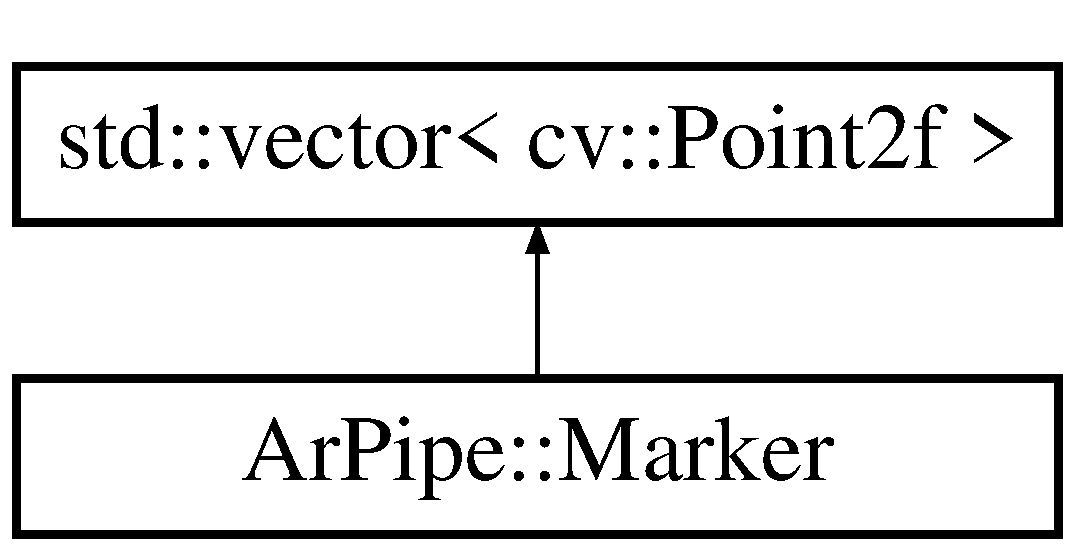
\includegraphics[height=2.000000cm]{d4/dc2/class_ar_pipe_1_1_marker}
\end{center}
\end{figure}
\subsection*{Veřejné metody}
\begin{DoxyCompactItemize}
\item 
\hypertarget{class_ar_pipe_1_1_marker_a3d32fab3fb0d1e3f1624fa1fc39e99b2}{{\bfseries Marker} (const \hyperlink{class_ar_pipe_1_1_marker}{Marker} \&M)}\label{d4/dc2/class_ar_pipe_1_1_marker_a3d32fab3fb0d1e3f1624fa1fc39e99b2}

\item 
\hypertarget{class_ar_pipe_1_1_marker_adf46f98ed52fa2d62d82a5558b0df012}{{\bfseries Marker} (const std\-::vector$<$ cv\-::\-Point2f $>$ \&corners, int \-\_\-id=-\/1)}\label{d4/dc2/class_ar_pipe_1_1_marker_adf46f98ed52fa2d62d82a5558b0df012}

\item 
bool \hyperlink{class_ar_pipe_1_1_marker_a5b2c8cec27db5cf9b26bb356542e8030}{is\-Valid} () const 
\item 
void \hyperlink{class_ar_pipe_1_1_marker_a7f9ac55816ba4e1ae1a991124042b648}{draw} (cv\-::\-Mat \&in, cv\-::\-Scalar color, int line\-Width=1, bool write\-Id=true) const 
\item 
void \hyperlink{class_ar_pipe_1_1_marker_adcb88ee0c2c59ceeb5ec706c18bae2b3}{calculate\-Extrinsics} (float marker\-Size, const \hyperlink{classaruco_1_1_camera_parameters}{aruco\-::\-Camera\-Parameters} \&C\-P)  throw (cv\-::\-Exception)
\item 
void \hyperlink{class_ar_pipe_1_1_marker_a2e6a3942e1e41b99b9051e654889fb85}{calculate\-Extrinsics} (float marker\-Size, cv\-::\-Mat Camera\-Matrix, cv\-::\-Mat Distorsion=cv\-::\-Mat())  throw (cv\-::\-Exception)
\item 
void \hyperlink{class_ar_pipe_1_1_marker_a5850ed86671d366d640d1c98b5dc4176}{gl\-Get\-Model\-View\-Matrix} (double modelview\-\_\-matrix\mbox{[}16\mbox{]})  throw (cv\-::\-Exception)
\item 
cv\-::\-Point2f \hyperlink{class_ar_pipe_1_1_marker_ae3529020574d565123af96b299a2dabc}{get\-Center} () const 
\item 
float \hyperlink{class_ar_pipe_1_1_marker_a067e6e118c4c310c104a039ed977bab5}{get\-Perimeter} () const 
\item 
float \hyperlink{class_ar_pipe_1_1_marker_ad7fc8a998dd21668d1f0bacf18c320b6}{get\-Area} () const 
\end{DoxyCompactItemize}
\subsection*{Veřejné atributy}
\begin{DoxyCompactItemize}
\item 
\hypertarget{class_ar_pipe_1_1_marker_a33f4be78f79f38e54d9b657ea3b12a72}{int {\bfseries id}}\label{d4/dc2/class_ar_pipe_1_1_marker_a33f4be78f79f38e54d9b657ea3b12a72}

\item 
\hypertarget{class_ar_pipe_1_1_marker_a4135dc060acf0aadee9633926d870faf}{float {\bfseries ssize}}\label{d4/dc2/class_ar_pipe_1_1_marker_a4135dc060acf0aadee9633926d870faf}

\item 
\hypertarget{class_ar_pipe_1_1_marker_a4aff6ef505f82a731320ed11ef25ca32}{cv\-::\-Mat {\bfseries Rvec}}\label{d4/dc2/class_ar_pipe_1_1_marker_a4aff6ef505f82a731320ed11ef25ca32}

\item 
\hypertarget{class_ar_pipe_1_1_marker_aa8c712e71d4b0ac13d99c3bdb028fa81}{cv\-::\-Mat {\bfseries Tvec}}\label{d4/dc2/class_ar_pipe_1_1_marker_aa8c712e71d4b0ac13d99c3bdb028fa81}

\end{DoxyCompactItemize}
\subsection*{Friends}
\begin{DoxyCompactItemize}
\item 
\hypertarget{class_ar_pipe_1_1_marker_a19de3d60e4cd6ddaf3df606158049a0c}{bool {\bfseries operator$<$} (const \hyperlink{class_ar_pipe_1_1_marker}{Marker} \&M1, const \hyperlink{class_ar_pipe_1_1_marker}{Marker} \&M2)}\label{d4/dc2/class_ar_pipe_1_1_marker_a19de3d60e4cd6ddaf3df606158049a0c}

\item 
\hypertarget{class_ar_pipe_1_1_marker_a191f20f61955983c0475ae4b141657ef}{ostream \& {\bfseries operator$<$$<$} (ostream \&str, const \hyperlink{class_ar_pipe_1_1_marker}{Marker} \&M)}\label{d4/dc2/class_ar_pipe_1_1_marker_a191f20f61955983c0475ae4b141657ef}

\end{DoxyCompactItemize}


\subsection{Detailní popis}
This class represents a marker. It is a vector of the fours corners ot the marker. 



\subsection{Dokumentace k metodám}
\hypertarget{class_ar_pipe_1_1_marker_adcb88ee0c2c59ceeb5ec706c18bae2b3}{\index{Ar\-Pipe\-::\-Marker@{Ar\-Pipe\-::\-Marker}!calculate\-Extrinsics@{calculate\-Extrinsics}}
\index{calculate\-Extrinsics@{calculate\-Extrinsics}!ArPipe::Marker@{Ar\-Pipe\-::\-Marker}}
\subsubsection[{calculate\-Extrinsics}]{\setlength{\rightskip}{0pt plus 5cm}void Ar\-Pipe\-::\-Marker\-::calculate\-Extrinsics (
\begin{DoxyParamCaption}
\item[{float}]{marker\-Size, }
\item[{const {\bf aruco\-::\-Camera\-Parameters} \&}]{C\-P}
\end{DoxyParamCaption}
)  throw (cv\-::\-Exception)}}\label{d4/dc2/class_ar_pipe_1_1_marker_adcb88ee0c2c59ceeb5ec706c18bae2b3}
Calculates the extrinsics (Rvec and Tvec) of the marker with respect to the camera 
\begin{DoxyParams}{Parametry}
{\em marker\-Size} & size of the marker side expressed in meters \\
\hline
{\em C\-P} & parmeters of the camera \\
\hline
\end{DoxyParams}
\hypertarget{class_ar_pipe_1_1_marker_a2e6a3942e1e41b99b9051e654889fb85}{\index{Ar\-Pipe\-::\-Marker@{Ar\-Pipe\-::\-Marker}!calculate\-Extrinsics@{calculate\-Extrinsics}}
\index{calculate\-Extrinsics@{calculate\-Extrinsics}!ArPipe::Marker@{Ar\-Pipe\-::\-Marker}}
\subsubsection[{calculate\-Extrinsics}]{\setlength{\rightskip}{0pt plus 5cm}void Ar\-Pipe\-::\-Marker\-::calculate\-Extrinsics (
\begin{DoxyParamCaption}
\item[{float}]{marker\-Size, }
\item[{cv\-::\-Mat}]{Camera\-Matrix, }
\item[{cv\-::\-Mat}]{Distorsion = {\ttfamily cv\-:\-:Mat()}}
\end{DoxyParamCaption}
)  throw (cv\-::\-Exception)}}\label{d4/dc2/class_ar_pipe_1_1_marker_a2e6a3942e1e41b99b9051e654889fb85}
Calculates the extrinsics (Rvec and Tvec) of the marker with respect to the camera 
\begin{DoxyParams}{Parametry}
{\em marker\-Size} & size of the marker side expressed in meters \\
\hline
{\em Camera\-Matrix} & matrix with camera parameters (fx,fy,cx,cy) \\
\hline
{\em Distorsion} & matrix with distorsion parameters (k1,k2,p1,p2) \\
\hline
\end{DoxyParams}
\hypertarget{class_ar_pipe_1_1_marker_a7f9ac55816ba4e1ae1a991124042b648}{\index{Ar\-Pipe\-::\-Marker@{Ar\-Pipe\-::\-Marker}!draw@{draw}}
\index{draw@{draw}!ArPipe::Marker@{Ar\-Pipe\-::\-Marker}}
\subsubsection[{draw}]{\setlength{\rightskip}{0pt plus 5cm}void Ar\-Pipe\-::\-Marker\-::draw (
\begin{DoxyParamCaption}
\item[{cv\-::\-Mat \&}]{in, }
\item[{cv\-::\-Scalar}]{color, }
\item[{int}]{line\-Width = {\ttfamily 1}, }
\item[{bool}]{write\-Id = {\ttfamily true}}
\end{DoxyParamCaption}
) const}}\label{d4/dc2/class_ar_pipe_1_1_marker_a7f9ac55816ba4e1ae1a991124042b648}
Draws this marker in the input image \hypertarget{class_ar_pipe_1_1_marker_ad7fc8a998dd21668d1f0bacf18c320b6}{\index{Ar\-Pipe\-::\-Marker@{Ar\-Pipe\-::\-Marker}!get\-Area@{get\-Area}}
\index{get\-Area@{get\-Area}!ArPipe::Marker@{Ar\-Pipe\-::\-Marker}}
\subsubsection[{get\-Area}]{\setlength{\rightskip}{0pt plus 5cm}float Ar\-Pipe\-::\-Marker\-::get\-Area (
\begin{DoxyParamCaption}
{}
\end{DoxyParamCaption}
) const}}\label{d4/dc2/class_ar_pipe_1_1_marker_ad7fc8a998dd21668d1f0bacf18c320b6}
Returns the area \hypertarget{class_ar_pipe_1_1_marker_ae3529020574d565123af96b299a2dabc}{\index{Ar\-Pipe\-::\-Marker@{Ar\-Pipe\-::\-Marker}!get\-Center@{get\-Center}}
\index{get\-Center@{get\-Center}!ArPipe::Marker@{Ar\-Pipe\-::\-Marker}}
\subsubsection[{get\-Center}]{\setlength{\rightskip}{0pt plus 5cm}cv\-::\-Point2f Ar\-Pipe\-::\-Marker\-::get\-Center (
\begin{DoxyParamCaption}
{}
\end{DoxyParamCaption}
) const}}\label{d4/dc2/class_ar_pipe_1_1_marker_ae3529020574d565123af96b299a2dabc}
Returns the centroid of the marker \hypertarget{class_ar_pipe_1_1_marker_a067e6e118c4c310c104a039ed977bab5}{\index{Ar\-Pipe\-::\-Marker@{Ar\-Pipe\-::\-Marker}!get\-Perimeter@{get\-Perimeter}}
\index{get\-Perimeter@{get\-Perimeter}!ArPipe::Marker@{Ar\-Pipe\-::\-Marker}}
\subsubsection[{get\-Perimeter}]{\setlength{\rightskip}{0pt plus 5cm}float Ar\-Pipe\-::\-Marker\-::get\-Perimeter (
\begin{DoxyParamCaption}
{}
\end{DoxyParamCaption}
) const}}\label{d4/dc2/class_ar_pipe_1_1_marker_a067e6e118c4c310c104a039ed977bab5}
Returns the perimeter of the marker \hypertarget{class_ar_pipe_1_1_marker_a5850ed86671d366d640d1c98b5dc4176}{\index{Ar\-Pipe\-::\-Marker@{Ar\-Pipe\-::\-Marker}!gl\-Get\-Model\-View\-Matrix@{gl\-Get\-Model\-View\-Matrix}}
\index{gl\-Get\-Model\-View\-Matrix@{gl\-Get\-Model\-View\-Matrix}!ArPipe::Marker@{Ar\-Pipe\-::\-Marker}}
\subsubsection[{gl\-Get\-Model\-View\-Matrix}]{\setlength{\rightskip}{0pt plus 5cm}void Ar\-Pipe\-::\-Marker\-::gl\-Get\-Model\-View\-Matrix (
\begin{DoxyParamCaption}
\item[{double}]{modelview\-\_\-matrix\mbox{[}16\mbox{]}}
\end{DoxyParamCaption}
)  throw (cv\-::\-Exception)}}\label{d4/dc2/class_ar_pipe_1_1_marker_a5850ed86671d366d640d1c98b5dc4176}
Given the extrinsic camera parameters returns the G\-L\-\_\-\-M\-O\-D\-E\-L\-V\-I\-E\-W matrix for opengl. Setting this matrix, the reference coordinate system will be set in this marker \hypertarget{class_ar_pipe_1_1_marker_a5b2c8cec27db5cf9b26bb356542e8030}{\index{Ar\-Pipe\-::\-Marker@{Ar\-Pipe\-::\-Marker}!is\-Valid@{is\-Valid}}
\index{is\-Valid@{is\-Valid}!ArPipe::Marker@{Ar\-Pipe\-::\-Marker}}
\subsubsection[{is\-Valid}]{\setlength{\rightskip}{0pt plus 5cm}bool Ar\-Pipe\-::\-Marker\-::is\-Valid (
\begin{DoxyParamCaption}
{}
\end{DoxyParamCaption}
) const\hspace{0.3cm}{\ttfamily [inline]}}}\label{d4/dc2/class_ar_pipe_1_1_marker_a5b2c8cec27db5cf9b26bb356542e8030}
Indicates if this object is valid 

Dokumentace pro tuto třídu byla generována z následujících souborů\-:\begin{DoxyCompactItemize}
\item 
Model/Marker.\-h\item 
Model/Marker.\-cpp\end{DoxyCompactItemize}

\hypertarget{class_ar_pipe_1_1_pipe_line}{\section{Dokumentace třídy Ar\-Pipe\-:\-:Pipe\-Line}
\label{de/d52/class_ar_pipe_1_1_pipe_line}\index{Ar\-Pipe\-::\-Pipe\-Line@{Ar\-Pipe\-::\-Pipe\-Line}}
}
Diagram dědičnosti pro třídu Ar\-Pipe\-:\-:Pipe\-Line\begin{figure}[H]
\begin{center}
\leavevmode
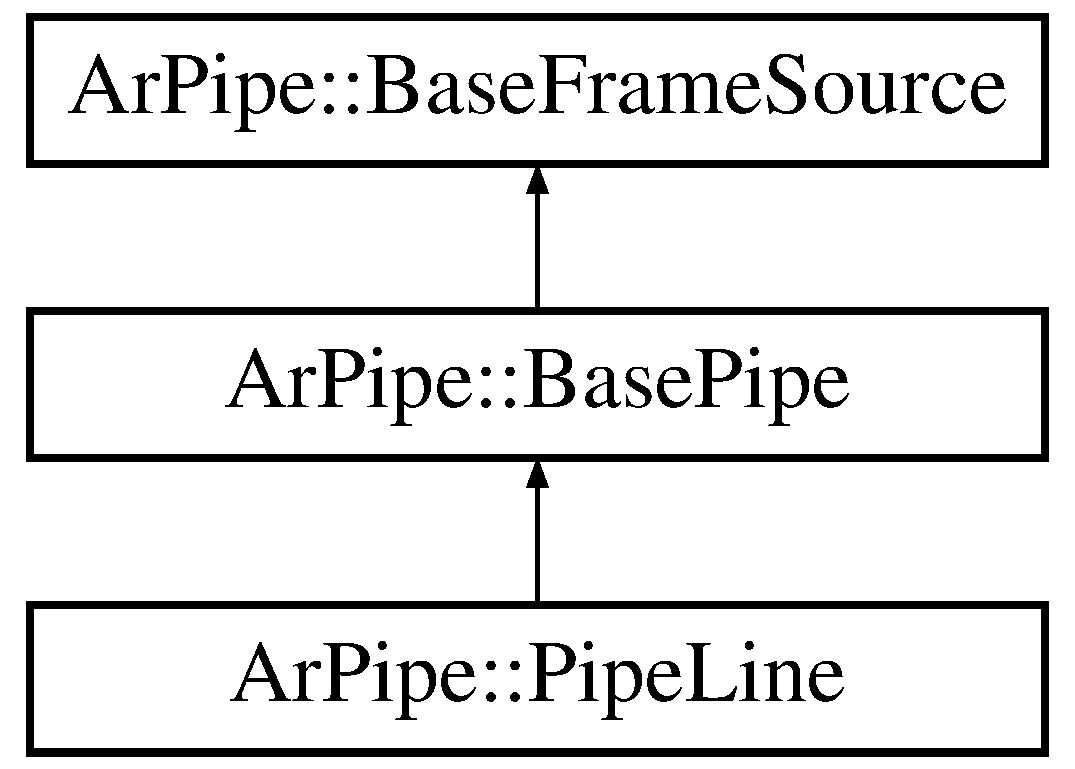
\includegraphics[height=3.000000cm]{de/d52/class_ar_pipe_1_1_pipe_line}
\end{center}
\end{figure}
\subsection*{Veřejné metody}
\begin{DoxyCompactItemize}
\item 
\hypertarget{class_ar_pipe_1_1_pipe_line_ac60335c05ee67c4c1b87a66a3a612a90}{{\bfseries Pipe\-Line} (\hyperlink{class_ar_pipe_1_1_base_frame_source}{Base\-Frame\-Source} $\ast$previous\-Pipe)}\label{de/d52/class_ar_pipe_1_1_pipe_line_ac60335c05ee67c4c1b87a66a3a612a90}

\item 
\hypertarget{class_ar_pipe_1_1_pipe_line_a452bd2085e1702ae8c3a2b8a3985fc9e}{void {\bfseries process\-Frame\-Container} (\hyperlink{class_ar_pipe_1_1_base_frame_container}{Base\-Frame\-Container} $\ast$frm, \hyperlink{class_ar_pipe_1_1_base_frame_source}{Base\-Frame\-Source} $\ast$frame\-Source)}\label{de/d52/class_ar_pipe_1_1_pipe_line_a452bd2085e1702ae8c3a2b8a3985fc9e}

\item 
\hypertarget{class_ar_pipe_1_1_pipe_line_af5041e1c1ac8b0fa1f5a2dbaad5c0294}{\hyperlink{class_ar_pipe_1_1_pipe_line}{Pipe\-Line} $\ast$ {\bfseries add\-Pipe} (\hyperlink{class_ar_pipe_1_1_base_pipe}{Base\-Pipe} $\ast$pipe)}\label{de/d52/class_ar_pipe_1_1_pipe_line_af5041e1c1ac8b0fa1f5a2dbaad5c0294}

\item 
\hypertarget{class_ar_pipe_1_1_pipe_line_a6a5140894b8c3c185aee4ed9ada5bdaf}{int {\bfseries get\-Count} ()}\label{de/d52/class_ar_pipe_1_1_pipe_line_a6a5140894b8c3c185aee4ed9ada5bdaf}

\item 
\hypertarget{class_ar_pipe_1_1_pipe_line_a5443fdee418ed714bfc08adaef54c093}{\hyperlink{class_ar_pipe_1_1_base_pipe}{Base\-Pipe} $\ast$ {\bfseries operator\mbox{[}$\,$\mbox{]}} (int i) const }\label{de/d52/class_ar_pipe_1_1_pipe_line_a5443fdee418ed714bfc08adaef54c093}

\item 
\hypertarget{class_ar_pipe_1_1_pipe_line_a5bd71d6d682f5c7ace3444122e66efce}{\hyperlink{class_ar_pipe_1_1_base_pipe}{Base\-Pipe} $\ast$\& {\bfseries operator\mbox{[}$\,$\mbox{]}} (int i)}\label{de/d52/class_ar_pipe_1_1_pipe_line_a5bd71d6d682f5c7ace3444122e66efce}

\end{DoxyCompactItemize}
\subsection*{Chráněné atributy}
\begin{DoxyCompactItemize}
\item 
\hypertarget{class_ar_pipe_1_1_pipe_line_a9e945633806868296d7fa8e1ef59e580}{std\-::vector$<$ \hyperlink{class_ar_pipe_1_1_base_pipe}{Base\-Pipe} $\ast$ $>$ {\bfseries sub\-Pipes}}\label{de/d52/class_ar_pipe_1_1_pipe_line_a9e945633806868296d7fa8e1ef59e580}

\end{DoxyCompactItemize}
\subsection*{Další zděděné členy}


Dokumentace pro tuto třídu byla generována z následujících souborů\-:\begin{DoxyCompactItemize}
\item 
Model/Pipe\-Line.\-h\item 
Model/Pipe\-Line.\-cpp\end{DoxyCompactItemize}

\hypertarget{class_ar_pipe_1_1_pipe_output_connector}{\section{Dokumentace třídy Ar\-Pipe\-:\-:Pipe\-Output\-Connector}
\label{da/d04/class_ar_pipe_1_1_pipe_output_connector}\index{Ar\-Pipe\-::\-Pipe\-Output\-Connector@{Ar\-Pipe\-::\-Pipe\-Output\-Connector}}
}
Diagram dědičnosti pro třídu Ar\-Pipe\-:\-:Pipe\-Output\-Connector\begin{figure}[H]
\begin{center}
\leavevmode
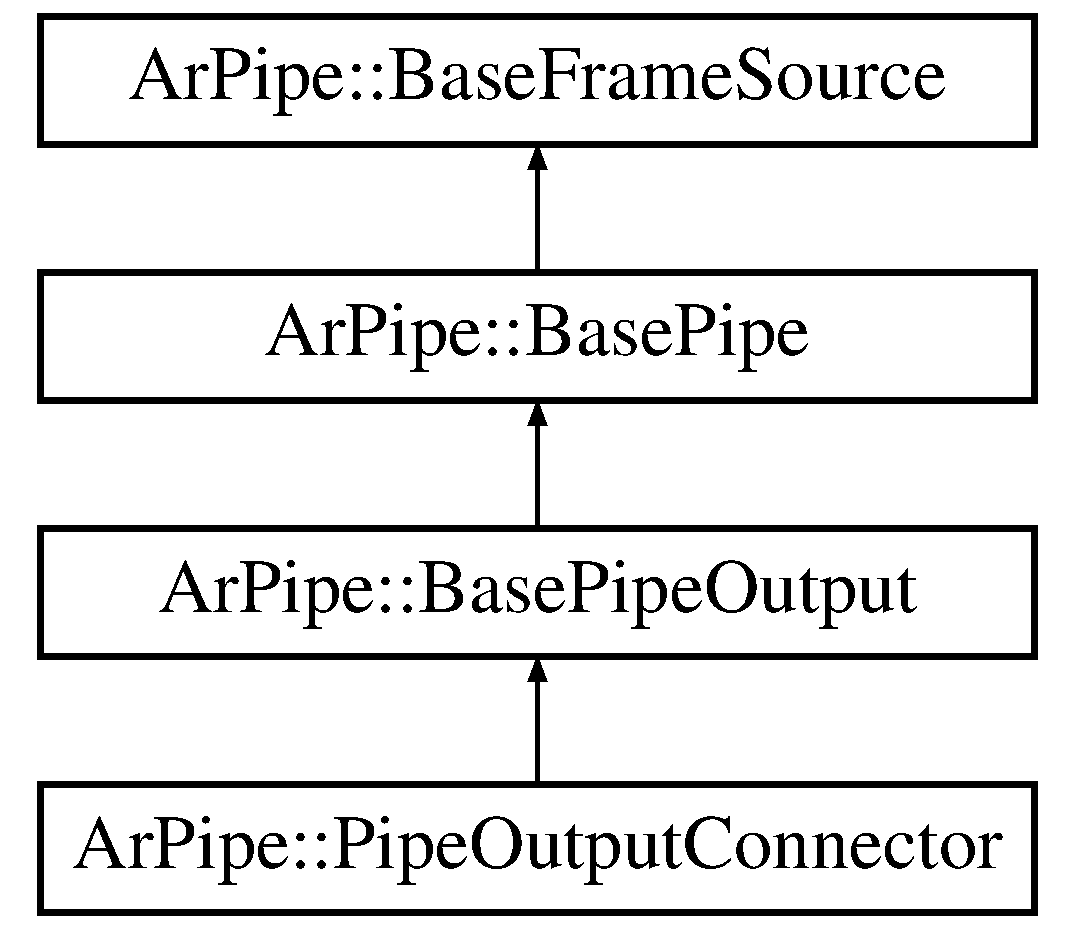
\includegraphics[height=4.000000cm]{da/d04/class_ar_pipe_1_1_pipe_output_connector}
\end{center}
\end{figure}
\subsection*{Veřejné metody}
\begin{DoxyCompactItemize}
\item 
\hypertarget{class_ar_pipe_1_1_pipe_output_connector_af59018bd78eed726aa662ef987ccf516}{void {\bfseries set\-On\-New\-Frame\-Container\-Callback} (void($\ast$callback)(\hyperlink{class_ar_pipe_1_1_base_frame_container}{Base\-Frame\-Container} $\ast$frm))}\label{da/d04/class_ar_pipe_1_1_pipe_output_connector_af59018bd78eed726aa662ef987ccf516}

\item 
\hypertarget{class_ar_pipe_1_1_pipe_output_connector_a00cec41506fb0cdcf2f0f6a215b9b91c}{void {\bfseries process\-Frame\-Container} (\hyperlink{class_ar_pipe_1_1_base_frame_container}{Base\-Frame\-Container} $\ast$frm, \hyperlink{class_ar_pipe_1_1_base_frame_source}{Base\-Frame\-Source} $\ast$frame\-Source)}\label{da/d04/class_ar_pipe_1_1_pipe_output_connector_a00cec41506fb0cdcf2f0f6a215b9b91c}

\end{DoxyCompactItemize}
\subsection*{Chráněné atributy}
\begin{DoxyCompactItemize}
\item 
\hypertarget{class_ar_pipe_1_1_pipe_output_connector_a02c6b01623f4c32967a42abfff1ac456}{void($\ast$ {\bfseries new\-Frame\-Callback} )(\hyperlink{class_ar_pipe_1_1_base_frame_container}{Base\-Frame\-Container} $\ast$frm)}\label{da/d04/class_ar_pipe_1_1_pipe_output_connector_a02c6b01623f4c32967a42abfff1ac456}

\end{DoxyCompactItemize}
\subsection*{Další zděděné členy}


Dokumentace pro tuto třídu byla generována z následujících souborů\-:\begin{DoxyCompactItemize}
\item 
i\-O\-S\-Connectors/Pipe\-Output\-Connector.\-h\item 
i\-O\-S\-Connectors/Pipe\-Output\-Connector.\-cpp\end{DoxyCompactItemize}

\hypertarget{class_ar_pipe_1_1_polar_rotate}{\section{Dokumentace třídy Ar\-Pipe\-:\-:Polar\-Rotate}
\label{da/dd5/class_ar_pipe_1_1_polar_rotate}\index{Ar\-Pipe\-::\-Polar\-Rotate@{Ar\-Pipe\-::\-Polar\-Rotate}}
}
Diagram dědičnosti pro třídu Ar\-Pipe\-:\-:Polar\-Rotate\begin{figure}[H]
\begin{center}
\leavevmode
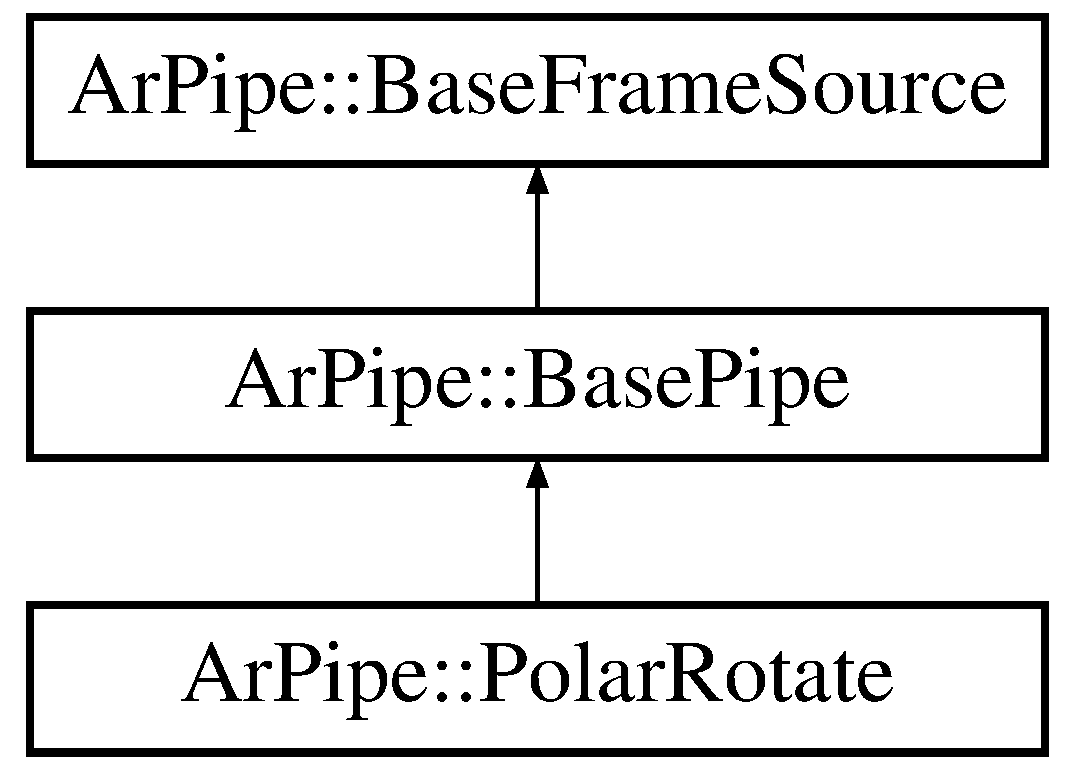
\includegraphics[height=3.000000cm]{da/dd5/class_ar_pipe_1_1_polar_rotate}
\end{center}
\end{figure}
\subsection*{Veřejné metody}
\begin{DoxyCompactItemize}
\item 
\hypertarget{class_ar_pipe_1_1_polar_rotate_a2c757268e7a78676fb11a72e7bd86e23}{{\bfseries Polar\-Rotate} (int degrees)}\label{da/dd5/class_ar_pipe_1_1_polar_rotate_a2c757268e7a78676fb11a72e7bd86e23}

\item 
\hypertarget{class_ar_pipe_1_1_polar_rotate_a7cd6e087a8065c73d5890b7a9aa7ed74}{\hyperlink{class_ar_pipe_1_1_polar_rotate}{Polar\-Rotate} $\ast$ {\bfseries set\-Deg} (int degrees)}\label{da/dd5/class_ar_pipe_1_1_polar_rotate_a7cd6e087a8065c73d5890b7a9aa7ed74}

\item 
\hypertarget{class_ar_pipe_1_1_polar_rotate_a2b1124780691c558e491c8aeb04e3a4c}{void {\bfseries process\-Frame\-Container} (\hyperlink{class_ar_pipe_1_1_base_frame_container}{Base\-Frame\-Container} $\ast$frm, \hyperlink{class_ar_pipe_1_1_base_frame_source}{Base\-Frame\-Source} $\ast$frame\-Source)}\label{da/dd5/class_ar_pipe_1_1_polar_rotate_a2b1124780691c558e491c8aeb04e3a4c}

\end{DoxyCompactItemize}
\subsection*{Statické veřejné metody}
\begin{DoxyCompactItemize}
\item 
\hypertarget{class_ar_pipe_1_1_polar_rotate_a2f0b3f1b219f81c69660725af826e9f8}{static \hyperlink{class_ar_pipe_1_1_polar_rotate}{Polar\-Rotate} $\ast$ {\bfseries init} (int degrees)}\label{da/dd5/class_ar_pipe_1_1_polar_rotate_a2f0b3f1b219f81c69660725af826e9f8}

\end{DoxyCompactItemize}
\subsection*{Chráněné atributy}
\begin{DoxyCompactItemize}
\item 
\hypertarget{class_ar_pipe_1_1_polar_rotate_a98cf74e421e5a40a214605b9dc884c64}{int {\bfseries deg}}\label{da/dd5/class_ar_pipe_1_1_polar_rotate_a98cf74e421e5a40a214605b9dc884c64}

\end{DoxyCompactItemize}


Dokumentace pro tuto třídu byla generována z následujících souborů\-:\begin{DoxyCompactItemize}
\item 
Pipes/\-Basic/Polar\-Rotate.\-h\item 
Pipes/\-Basic/Polar\-Rotate.\-cpp\end{DoxyCompactItemize}

\hypertarget{class_ar_pipe_1_1_shapes}{\section{Dokumentace třídy Ar\-Pipe\-:\-:Shapes}
\label{d0/db7/class_ar_pipe_1_1_shapes}\index{Ar\-Pipe\-::\-Shapes@{Ar\-Pipe\-::\-Shapes}}
}
\subsection*{Veřejné metody}
\begin{DoxyCompactItemize}
\item 
\hypertarget{class_ar_pipe_1_1_shapes_ae21c9a2c3484f9a72d45306314839a5d}{std\-::vector$<$ std\-::vector\\*
$<$ cv\-::\-Point $>$ $>$ \& {\bfseries get\-Contours} ()}\label{d0/db7/class_ar_pipe_1_1_shapes_ae21c9a2c3484f9a72d45306314839a5d}

\item 
\hypertarget{class_ar_pipe_1_1_shapes_adc073e4c1fb75f3846538376f6e2fbea}{std\-::vector$<$ cv\-::\-Vec4i $>$ \& {\bfseries get\-Hierarchy} ()}\label{d0/db7/class_ar_pipe_1_1_shapes_adc073e4c1fb75f3846538376f6e2fbea}

\item 
\hypertarget{class_ar_pipe_1_1_shapes_a7b781881afb34d5b8cb2e42809549814}{std\-::vector$<$ \hyperlink{class_ar_pipe_1_1_marker}{Marker} $>$ \& {\bfseries get\-Markers} ()}\label{d0/db7/class_ar_pipe_1_1_shapes_a7b781881afb34d5b8cb2e42809549814}

\end{DoxyCompactItemize}
\subsection*{Chráněné atributy}
\begin{DoxyCompactItemize}
\item 
\hypertarget{class_ar_pipe_1_1_shapes_a0d17027098bad1d733ab955cc9cbe82d}{std\-::vector$<$ std\-::vector\\*
$<$ cv\-::\-Point $>$ $>$ {\bfseries contours}}\label{d0/db7/class_ar_pipe_1_1_shapes_a0d17027098bad1d733ab955cc9cbe82d}

\item 
\hypertarget{class_ar_pipe_1_1_shapes_af157d96b7cf4de75f130a0247d94ab50}{std\-::vector$<$ cv\-::\-Vec4i $>$ {\bfseries hierarchy}}\label{d0/db7/class_ar_pipe_1_1_shapes_af157d96b7cf4de75f130a0247d94ab50}

\item 
\hypertarget{class_ar_pipe_1_1_shapes_ac8d350477cc3a1ba0ad402efdd50cac4}{std\-::vector$<$ \hyperlink{class_ar_pipe_1_1_marker}{Marker} $>$ {\bfseries markers}}\label{d0/db7/class_ar_pipe_1_1_shapes_ac8d350477cc3a1ba0ad402efdd50cac4}

\end{DoxyCompactItemize}


Dokumentace pro tuto třídu byla generována z následujícího souboru\-:\begin{DoxyCompactItemize}
\item 
Model/Shapes.\-h\end{DoxyCompactItemize}

\hypertarget{class_ar_pipe_1_1_square_marker_detector}{\section{Dokumentace třídy Ar\-Pipe\-:\-:Square\-Marker\-Detector}
\label{d1/d0f/class_ar_pipe_1_1_square_marker_detector}\index{Ar\-Pipe\-::\-Square\-Marker\-Detector@{Ar\-Pipe\-::\-Square\-Marker\-Detector}}
}
Diagram dědičnosti pro třídu Ar\-Pipe\-:\-:Square\-Marker\-Detector\begin{figure}[H]
\begin{center}
\leavevmode
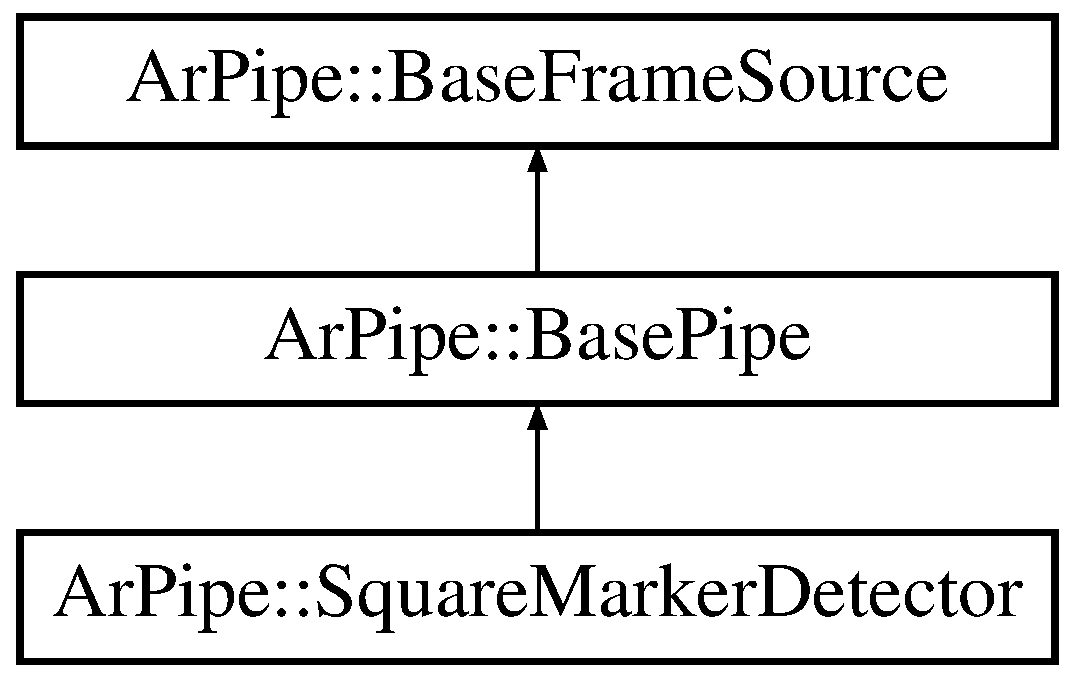
\includegraphics[height=3.000000cm]{d1/d0f/class_ar_pipe_1_1_square_marker_detector}
\end{center}
\end{figure}
\subsection*{Veřejné metody}
\begin{DoxyCompactItemize}
\item 
\hypertarget{class_ar_pipe_1_1_square_marker_detector_a29fcbdaf7a5783c427d0962c798239bc}{{\bfseries Square\-Marker\-Detector} (\hyperlink{class_ar_pipe_1_1_base_frame_source}{Base\-Frame\-Source} $\ast$previous\-Pipe)}\label{d1/d0f/class_ar_pipe_1_1_square_marker_detector_a29fcbdaf7a5783c427d0962c798239bc}

\item 
void \hyperlink{class_ar_pipe_1_1_square_marker_detector_aab270ab9b57d8a1429562565c1cc2965}{process\-Frame\-Container} (\hyperlink{class_ar_pipe_1_1_base_frame_container}{Base\-Frame\-Container} $\ast$frm, \hyperlink{class_ar_pipe_1_1_base_frame_source}{Base\-Frame\-Source} $\ast$frame\-Source)
\end{DoxyCompactItemize}
\subsection*{Statické veřejné metody}
\begin{DoxyCompactItemize}
\item 
\hypertarget{class_ar_pipe_1_1_square_marker_detector_adedf817c2685712f3bcb05edeeb599ae}{static \hyperlink{class_ar_pipe_1_1_square_marker_detector}{Square\-Marker\-Detector} $\ast$ {\bfseries init} ()}\label{d1/d0f/class_ar_pipe_1_1_square_marker_detector_adedf817c2685712f3bcb05edeeb599ae}

\end{DoxyCompactItemize}
\subsection*{Další zděděné členy}


\subsection{Dokumentace k metodám}
\hypertarget{class_ar_pipe_1_1_square_marker_detector_aab270ab9b57d8a1429562565c1cc2965}{\index{Ar\-Pipe\-::\-Square\-Marker\-Detector@{Ar\-Pipe\-::\-Square\-Marker\-Detector}!process\-Frame\-Container@{process\-Frame\-Container}}
\index{process\-Frame\-Container@{process\-Frame\-Container}!ArPipe::SquareMarkerDetector@{Ar\-Pipe\-::\-Square\-Marker\-Detector}}
\subsubsection[{process\-Frame\-Container}]{\setlength{\rightskip}{0pt plus 5cm}void Ar\-Pipe\-::\-Square\-Marker\-Detector\-::process\-Frame\-Container (
\begin{DoxyParamCaption}
\item[{{\bf Base\-Frame\-Container} $\ast$}]{frm, }
\item[{{\bf Base\-Frame\-Source} $\ast$}]{frame\-Source}
\end{DoxyParamCaption}
)\hspace{0.3cm}{\ttfamily [virtual]}}}\label{d1/d0f/class_ar_pipe_1_1_square_marker_detector_aab270ab9b57d8a1429562565c1cc2965}
identify the markers

refine the corner location if desired

detect the position of detected markers if desired 

Reimplementuje stejnojmenný prvek z \hyperlink{class_ar_pipe_1_1_base_pipe}{Ar\-Pipe\-::\-Base\-Pipe}.



Dokumentace pro tuto třídu byla generována z následujících souborů\-:\begin{DoxyCompactItemize}
\item 
Pipes/\-Detectors/Square\-Marker\-Detector.\-h\item 
Pipes/\-Detectors/Square\-Marker\-Detector.\-cpp\end{DoxyCompactItemize}

\hypertarget{class_ar_pipe_1_1_threshold}{\section{Dokumentace třídy Ar\-Pipe\-:\-:Threshold}
\label{d8/df3/class_ar_pipe_1_1_threshold}\index{Ar\-Pipe\-::\-Threshold@{Ar\-Pipe\-::\-Threshold}}
}
Diagram dědičnosti pro třídu Ar\-Pipe\-:\-:Threshold\begin{figure}[H]
\begin{center}
\leavevmode
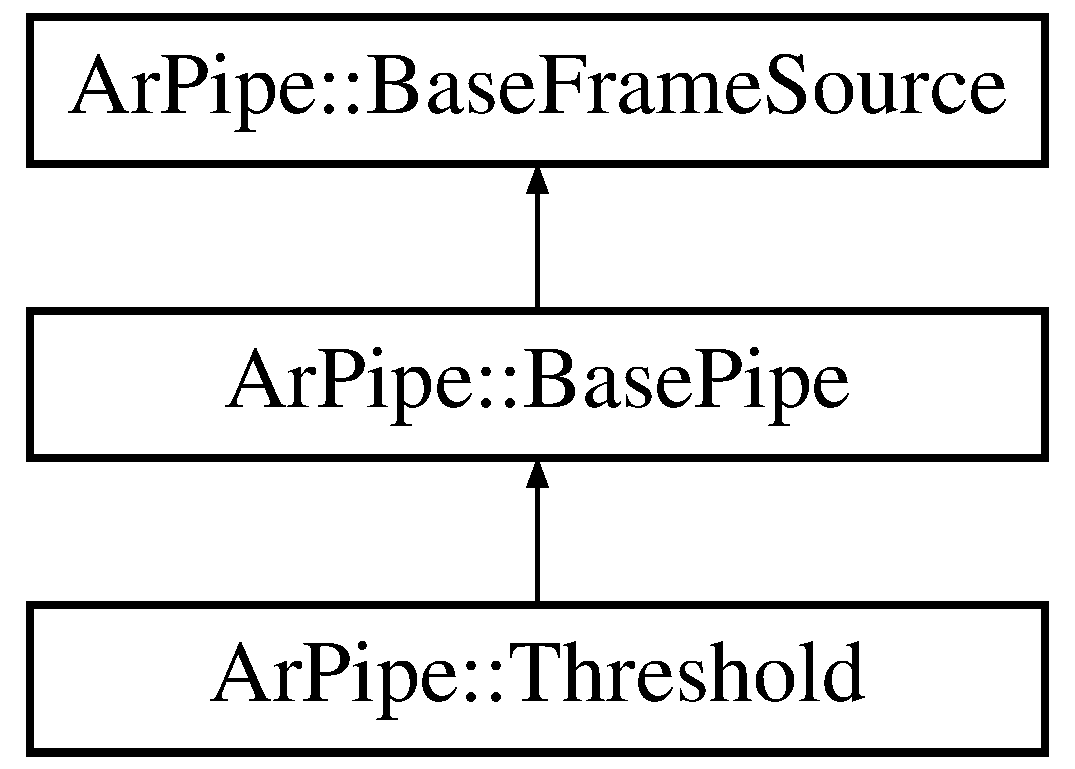
\includegraphics[height=3.000000cm]{d8/df3/class_ar_pipe_1_1_threshold}
\end{center}
\end{figure}
\subsection*{Veřejné metody}
\begin{DoxyCompactItemize}
\item 
\hypertarget{class_ar_pipe_1_1_threshold_ae714b2f34950e11dbd5ce399bf7da5fc}{{\bfseries Threshold} (\hyperlink{class_ar_pipe_1_1_base_frame_source}{Base\-Frame\-Source} $\ast$previous\-Pipe)}\label{d8/df3/class_ar_pipe_1_1_threshold_ae714b2f34950e11dbd5ce399bf7da5fc}

\item 
\hypertarget{class_ar_pipe_1_1_threshold_a6cff62cb7bce78cf9d741c286b6dbb9e}{void {\bfseries process\-Frame\-Container} (\hyperlink{class_ar_pipe_1_1_base_frame_container}{Base\-Frame\-Container} $\ast$frm, \hyperlink{class_ar_pipe_1_1_base_frame_source}{Base\-Frame\-Source} $\ast$frame\-Source)}\label{d8/df3/class_ar_pipe_1_1_threshold_a6cff62cb7bce78cf9d741c286b6dbb9e}

\item 
\hypertarget{class_ar_pipe_1_1_threshold_aec36111ebf06dec612aeec433483db60}{void {\bfseries set\-Type} (int type\-Const)}\label{d8/df3/class_ar_pipe_1_1_threshold_aec36111ebf06dec612aeec433483db60}

\item 
\hypertarget{class_ar_pipe_1_1_threshold_af1ba0f9421d1dfd91392461d55ddc6d6}{int {\bfseries get\-Type} ()}\label{d8/df3/class_ar_pipe_1_1_threshold_af1ba0f9421d1dfd91392461d55ddc6d6}

\item 
\hypertarget{class_ar_pipe_1_1_threshold_a3cc5112ebe234f173d838241f5d34642}{\hyperlink{class_ar_pipe_1_1_threshold}{Threshold} $\ast$ {\bfseries set\-Thresh} (double tresh\-Val)}\label{d8/df3/class_ar_pipe_1_1_threshold_a3cc5112ebe234f173d838241f5d34642}

\item 
\hypertarget{class_ar_pipe_1_1_threshold_abbdd0700d58ecf1a0523b07924979441}{double {\bfseries get\-Thresh} ()}\label{d8/df3/class_ar_pipe_1_1_threshold_abbdd0700d58ecf1a0523b07924979441}

\item 
\hypertarget{class_ar_pipe_1_1_threshold_a406a70d7ba3e40ce169798ecb83f2a09}{\hyperlink{class_ar_pipe_1_1_threshold}{Threshold} $\ast$ {\bfseries set\-Max\-Val} (double max)}\label{d8/df3/class_ar_pipe_1_1_threshold_a406a70d7ba3e40ce169798ecb83f2a09}

\item 
\hypertarget{class_ar_pipe_1_1_threshold_a889342cf5ddba9fa2a5b778b3a609786}{double {\bfseries get\-Max\-Val} ()}\label{d8/df3/class_ar_pipe_1_1_threshold_a889342cf5ddba9fa2a5b778b3a609786}

\item 
\hypertarget{class_ar_pipe_1_1_threshold_adf31e7f82d00ebedaeae14e52dd7f2d9}{\hyperlink{class_ar_pipe_1_1_threshold}{Threshold} $\ast$ {\bfseries set\-Auto\-Max} ()}\label{d8/df3/class_ar_pipe_1_1_threshold_adf31e7f82d00ebedaeae14e52dd7f2d9}

\item 
\hypertarget{class_ar_pipe_1_1_threshold_a22430d64c5f9193b832accce657b3bd3}{\hyperlink{class_ar_pipe_1_1_threshold}{Threshold} $\ast$ {\bfseries set\-Adaptive} (bool inverted)}\label{d8/df3/class_ar_pipe_1_1_threshold_a22430d64c5f9193b832accce657b3bd3}

\item 
\hypertarget{class_ar_pipe_1_1_threshold_aea0b86e19342a02490536d2b84703f7f}{\hyperlink{class_ar_pipe_1_1_threshold}{Threshold} $\ast$ {\bfseries set\-Type\-Binary} (bool inverted)}\label{d8/df3/class_ar_pipe_1_1_threshold_aea0b86e19342a02490536d2b84703f7f}

\item 
\hypertarget{class_ar_pipe_1_1_threshold_ab69e91b9d19b8450e03700b09e9e0cf1}{\hyperlink{class_ar_pipe_1_1_threshold}{Threshold} $\ast$ {\bfseries set\-Type\-Binary} (bool inverted, double max)}\label{d8/df3/class_ar_pipe_1_1_threshold_ab69e91b9d19b8450e03700b09e9e0cf1}

\item 
\hypertarget{class_ar_pipe_1_1_threshold_ae5cfed4406d87a838e80b0fa19731cc8}{\hyperlink{class_ar_pipe_1_1_threshold}{Threshold} $\ast$ {\bfseries set\-Type\-To\-Zero} (bool inverted)}\label{d8/df3/class_ar_pipe_1_1_threshold_ae5cfed4406d87a838e80b0fa19731cc8}

\item 
\hypertarget{class_ar_pipe_1_1_threshold_aec3481501482f08c9dd99420808c8871}{\hyperlink{class_ar_pipe_1_1_threshold}{Threshold} $\ast$ {\bfseries set\-Type\-Truncated} ()}\label{d8/df3/class_ar_pipe_1_1_threshold_aec3481501482f08c9dd99420808c8871}

\item 
\hypertarget{class_ar_pipe_1_1_threshold_ad44bb73524e880a38a18a174fa1aeefa}{\hyperlink{class_ar_pipe_1_1_threshold}{Threshold} $\ast$ {\bfseries set\-Adaptive\-Block\-Radius} (int size)}\label{d8/df3/class_ar_pipe_1_1_threshold_ad44bb73524e880a38a18a174fa1aeefa}

\item 
\hypertarget{class_ar_pipe_1_1_threshold_a67fe77dad4fffe65d7d659c3ebbeb4bb}{\hyperlink{class_ar_pipe_1_1_threshold}{Threshold} $\ast$ {\bfseries set\-Adaptive\-Method\-Mean} ()}\label{d8/df3/class_ar_pipe_1_1_threshold_a67fe77dad4fffe65d7d659c3ebbeb4bb}

\item 
\hypertarget{class_ar_pipe_1_1_threshold_a1b01cf27676585d8d91d37ac31e0b9fa}{\hyperlink{class_ar_pipe_1_1_threshold}{Threshold} $\ast$ {\bfseries set\-Adaptive\-Method\-Gaussian} ()}\label{d8/df3/class_ar_pipe_1_1_threshold_a1b01cf27676585d8d91d37ac31e0b9fa}

\end{DoxyCompactItemize}
\subsection*{Statické veřejné metody}
\begin{DoxyCompactItemize}
\item 
\hypertarget{class_ar_pipe_1_1_threshold_a0e2a97fce2b23771a6fbbc1abd379dca}{static \hyperlink{class_ar_pipe_1_1_threshold}{Threshold} $\ast$ {\bfseries init} ()}\label{d8/df3/class_ar_pipe_1_1_threshold_a0e2a97fce2b23771a6fbbc1abd379dca}

\end{DoxyCompactItemize}
\subsection*{Chráněné metody}
\begin{DoxyCompactItemize}
\item 
\hypertarget{class_ar_pipe_1_1_threshold_a26d5f2edf5040d67bc9dcf2630f2e6d4}{double {\bfseries get\-Calced\-Max\-Value} (\hyperlink{class_ar_pipe_1_1_frame}{Frame} $\ast$const mat)}\label{d8/df3/class_ar_pipe_1_1_threshold_a26d5f2edf5040d67bc9dcf2630f2e6d4}

\end{DoxyCompactItemize}
\subsection*{Chráněné atributy}
\begin{DoxyCompactItemize}
\item 
\hypertarget{class_ar_pipe_1_1_threshold_ab3cd04c648cc5f96b04e6c2ceabe49c8}{bool {\bfseries adaptive}}\label{d8/df3/class_ar_pipe_1_1_threshold_ab3cd04c648cc5f96b04e6c2ceabe49c8}

\item 
\hypertarget{class_ar_pipe_1_1_threshold_ae9ee1f7a8848a82c4bf25465fc17b7c6}{bool {\bfseries auto\-Max}}\label{d8/df3/class_ar_pipe_1_1_threshold_ae9ee1f7a8848a82c4bf25465fc17b7c6}

\item 
\hypertarget{class_ar_pipe_1_1_threshold_aa7413e3cebd23047479e553755bd2cff}{double {\bfseries thresh}}\label{d8/df3/class_ar_pipe_1_1_threshold_aa7413e3cebd23047479e553755bd2cff}

\item 
\hypertarget{class_ar_pipe_1_1_threshold_a45b73051f1cfb52e3aa2a09c67911b63}{double {\bfseries maxval}}\label{d8/df3/class_ar_pipe_1_1_threshold_a45b73051f1cfb52e3aa2a09c67911b63}

\item 
\hypertarget{class_ar_pipe_1_1_threshold_a1b30d543651f4a3895c9afd566b57a91}{int {\bfseries type}}\label{d8/df3/class_ar_pipe_1_1_threshold_a1b30d543651f4a3895c9afd566b57a91}

\item 
\hypertarget{class_ar_pipe_1_1_threshold_aa591a8a887a078d0209694628abab758}{int {\bfseries block\-Size}}\label{d8/df3/class_ar_pipe_1_1_threshold_aa591a8a887a078d0209694628abab758}

\item 
\hypertarget{class_ar_pipe_1_1_threshold_a784900859a1295579ee7c792e986ae52}{int {\bfseries adaptive\-Method}}\label{d8/df3/class_ar_pipe_1_1_threshold_a784900859a1295579ee7c792e986ae52}

\end{DoxyCompactItemize}


Dokumentace pro tuto třídu byla generována z následujících souborů\-:\begin{DoxyCompactItemize}
\item 
Pipes/\-Effects/Threshold.\-h\item 
Pipes/\-Effects/Threshold.\-cpp\end{DoxyCompactItemize}

\addcontentsline{toc}{part}{Rejstřík}
\printindex
\end{document}
